\documentclass[11pt,twoside,openright]{memoir}

%% IMPORTS
\usepackage{amsmath,amssymb,amsfonts,amsthm}               % math symbols
\usepackage[answerdelayed,lastexercise]{exercise}          % exercises
\usepackage{float}
\usepackage{listings}                                      % source code
\usepackage{pgfplots}                                      % plotting
\usepackage{tkz-euclide}                                   % tikz drawings
\usepackage{ulem}
\usepackage{xcolor}                                        % custom colors
\usepackage{xlop}                                          % arithmetic
% must be loaded last as it clashes with other packages
\usepackage{hyperref}                                      % http links

%% SETUP
% - PGF plots
\usepgfplotslibrary{statistics}
% - colors
\hypersetup{
    colorlinks,
    citecolor=black,
    filecolor=black,
    linkcolor=black,
    urlcolor=black
}
\restylefloat{table}
\usetkzobj{all}
% - ams theorem Styles
\newtheorem{theorem}{Theorem}[section]
\newtheorem{lemma}[theorem]{Lemma}
\newtheorem{proposition}[theorem]{Proposition}
\newtheorem{corollary}[theorem]{Corollary}
% - ams definition Styles
\theoremstyle{definition}
\newtheorem{definition}{Definition}[section]
\newtheorem{example}{Example}[section]
\theoremstyle{remark}
\newtheorem{remark}{Remark}
% redefine commands
\renewcommand{\deg}{\ensuremath{^{\circ}}\xspace}
% - custom commands
\newcommand{\rom}[1]{\uppercase\expandafter{\romannumeral #1\relax}}
\newcommand{\rad}{\deg}
\newcommand\showdiv[1]{\overline{\smash{)}#1}}
\newcommand\ph[1]{\textcolor{white}{#1}}
\newcommand{\myindent}{\hspace{0.45cm}}
% memoir class setup
\makepagenote
\renewcommand*{\notedivision}{\section{\notesname}} % page notes in same chapter
\renewcommand*{\pagenotesubhead}[3]{} % #1-chapname, #2-chapnum, #3-chaptitle removed
\renewcommand*{\pagenotesubheadstarred}[3]{} % chapname, chaptitle removed

% index
\makeindex
%% use \gls{} or \Gls to reference singular names
% use \glspl or \Glspl to reference plural names

% TODO missing from glossary
% Domain and CoDomain
% Sujective, Bijective and injective
% Monomial, binomial, polynomial
% Quadratic equations
% Product, Factors
% DC
% DB
%* Cashflow
%* PV
%* PMT
%* FV
%* Principle (capital amount)
% - the amount lent or borrowed is usually refered to as the principle or capital amount
%* **Market value:**
%* **Provision (hensættelse):** an account which records a present liability of the plan provider to its policy holders.
% coupon rate
% bond equivalent yield
% SPV (stochastic present value)
% ABO (accumulated benefit obligation)
% PBO (projected benefit obligation)
% Annuity
% LumpSum
% Brownian motion
% Gompertz-Makeham mortality
% Put options
% Utility function of wealth
% Bernoulli random variable
% Manifolds

\glsentry{associativity}{operation is associativ if within
an expression containing two or more occurrences in a row of the same
associative operator, the order in which the operations are performed
does not matter as long as the sequence of the operands is not changed.}

\glsentry{axiom}{}

\glsentry{cohort}{A group of subjects who have shared a particular
event together during a particular time span (e.g., people born in Europe
between 1918 and 1939; survivors of an aircrash; truck drivers who smoked
between age 30 and 40)}

\glsentry{commutativity}{Commutativity operation is commutative if
changing the order of the operands does not change the result.}

\glsentry{constant}{a number, term or expression that doesn't change. If
$y = x + 7$ then 7 is a constant. The area of a circle equals $2\pi r$ where
$r$ is the radius (a variable), and $\pi$ is a constant.}

\glsentry{factor}{a number or expression that divides exactly into
another number or expression. 1,2 and 5 are factors of 10; x and (2x + 3)
are factors of 2x2 + 3x because x multiplied by (2x + 3) = 2x2 + 3x.}

\glsentry{fraction}{a number such as 1/2, 2/3, 17/2. Can also be written
with a horizontal line, eg . The number above the line (called the
numerator) is divided by the number below the line (called the
denominator).}

\glsentry{irrational number}{A number that is not rational, eg $\pi$,
Euler's number e.}

\glsentry{linear equation}{A algebraic expression, usually of the form
\[
ax = b
\]
in which each term is either a constant or the product of a constant and
(the first power of) a single variable (that is no variables in the
expression contains exponents, like the $2$ in $x^2$, square roots,
cube roots, etc.)}

\glsentry{measure}{A measure on a set is a systematic way to assign a
number to each suitable subset of that set, intuitively interpreted as
its size. In this sense, a measure is a generalisation of the concepts
of length, area, and volume}

\glsentry{QED}{\emph{Quod erat demonstrandum}, Latin for
\emph{which was to be proved}}

\glsentry{rational expressions}{A expression
involving fractions of polynomials such as $\frac{x-1}{x^2 + 12}$.}

\glsentry{rational number}{A number that can be made by dividing one
integer by another, eg 1/2, 5/7, 12/108, 12/1.}

\glsentry{real number}{the normal numbers we use, including decimals,
fractions, integers, negative numbers, positive numbers, irrational
numbers, etc. They are called real because they aren't complex numbers
(numbers that involve the square root of -1)}

\glsentry{square}{the square of a number is the number multiplied by
itself, eg 5 squared = 52 = 25}

\glsentry{square root}{the square root of a number is a number that when
multiplied by itself gives the original number. The square root of 36 is
6. The square root symbol is , so .}

\glsentry{statement}{\emph{If P, then Q}, where its
\textbf{converse} has the following form: \emph{if Q, then P}}

\glsentry{term}{}

\glsentry{variable}{a quantity that may change, eg the circumference of a
circle equals 2πr where π (pi) is a constant and r, the radius, is a
variable.}


% configure title page
\makeatletter
\def\maketitle{%
  \null
  \thispagestyle{empty}%
  \vfill
  \begin{center}\leavevmode
    \normalfont
    {\LARGE\raggedleft \@author\par}%
    \hrulefill\par
    {\huge\raggedright \@title\par}%
    \vskip 1cm
    {\Large\raggedright Volume 1\par}%
    \vskip 0.5cm
    {\Large\raggedright Fundemental Mathematics \par}%
    \vskip 0.5cm
    {\Large\raggedright First Edition \par}%
  \end{center}%
  \vfill
  \null
  \cleardoublepage
  }
\makeatother
\author{Lars Tackmann}
\title{Concepts of Mathematics}

% begin document
\begin{document}

% title page
\let\cleardoublepage\clearpage
\maketitle

% table of contents
\tableofcontents
\pagenumbering{arabic}

% book layout
\chapter{Introduction}
It has been said that the typical theorem in mathematics states that something you do not understand is equal to something else you cannot compute. There is a kernel of truth in this joke, since the rigor required when doing mathematical research has found is way into every nook and corner of every textbook and thereby to a large extend rendered them unreadable to all, except fairly expert mathematicians; and even these usually disdain from reading such texts cover to cover. The value of mathematical rigor is not in the question; but such works are condemned to remain works of reference, to be consulted, not read.

This is unfortunate since many people derive great happiness from dabbling with a little mathematics; just consider the many people who daily tries to solve news paper Sudoku puzzles. Such activities implies that many people enjoys the pleasures of the mind and might even find a little mathematical education fulfilling. However it would be foolish not to acknowledge the complexity of modern mathematics. After all Andrew Wiles incredible proof of Fermat's Last Theorem or Abel's remarkable proof of the in-solvability of general higher degree equations eluded many of the worlds best mathematicians for centuries. Such gems are usually only available to the person equipped with a sharp mind, a fairly developed bag of mathematical tools and a certain intellectual maturity. What I propose here is a book that will build up enough knowledge to show the proofs of some of the greatest theorems in the history of mathematics; from Hippocrates Quadrature of the Lune to Lindeman's proof that $\pi$ is transcendental. I have sought to make the text completely self contained, so the reader will be taken from simple arithmetic to measure theory and game theory.

The mathematical mature person is right to ask if such an bold attempt is not futile and perhaps its author is a bit naive. There goes a story that the great physicist Richard Feynman was once asked by a Caltech faculty member to explain why spin $1/2$ particles obey the \index{Fermi-Dirac statistics}. He nodded and said, "I'll prepare a freshman lecture on it". But a few days later he returned and said. "You know, I couldn't do it, I couldn't reduce it to freshman level. That means we really don't understand it." Just as Feynman found out this author has also had to abandon a number of otherwise interesting subjects due to the complexity of conveying them within a reasonable span of pages.

The text includes a number of exercises along with answers to every one (at least briefly). I am a firm believer in learning-by-looking, also known as cheating, and thus I encourage the reader to give each problem his best shot, then check the answer. If correct then move on to a more advanced problem, if not then study the provided solution and try to solve a similar problem. If you are stuck then don't panic I have included an entire chapter devoted to the fine art of problem solving and mathematical proof.

The subject presented here is not laid out in the usual chronological manner, instead I have sought to build up mathematics as a logical progression of ever more complex ideas. Therefor instead of focusing on historical order I have strived instead to provide the clearest proofs; so for example, instead of \index{Oresme}'s original verbal proof of the divergence of \index{harmonic series} I have instead included a new simple algebraic proof. At other times the original proof is so beautiful or provide a vital lessons in mathematical reasoning that I let it's author speak directly (such as Euclid's proof of the Pyteagorian theorem).

The knowledge and proofs contained herein is taken from a multitude of sources, many have been rewritten or reordered so to make them more accessible, but often one finds mathematics written with such breathtaking clarity as so to render any further attempt upon simplification impossible. In these cases the information is simply restated and put in context. 

\indent Mathematics is utility and its usage is spread far and wide; from logical reason about programming languages to the physical sciences. So stories about its usages is included whenever I have found it fitting. At the same time mathematics is also history, from Archimedes war machines used against the intruding romans to everyday stories such as Newton's remark that he "do not like to be teased by foreigners about mathematical things". In the end all that I hope to achieve is to shine a little light on the fascinating field of human creativity known as mathematics, to hopefully illustrate the meaning of the the great philosopher Spinoza's words, when he said that "God is a mathematician". \\
\flushright Lars Tackmann \\ Copenhagen, Denmark\flushleft



\mainmatter
%\part{Fundemental Mathematics}
\chapter{Mathematical foundations}

\epigraph{You just keep pushing. You just keep pushing. I made every mistake that could be made. But I just kept pushing.}{Rene Descartes}

\section{Problem solving}
\subsection{Word problems}
"A bat and ball, together, cost a total of $1.10$ and the bat costs $1$ more than the ball. How much is the ball?" The wrong answer is the one that roughly one in every two people blurts out: 10 cents. The correct answer is 5 cents, since only with a bat worth $1.05$ and a ball worth $5$ pence are both conditions satisfied.

\subsection{Problem solving checklist}

\section{Proving theorems}
% TODO http://jeremykun.com/2015/06/08/methods-of-proof-diagonalization/
\subsection{Proof by induction}
\subsection{Proof checklist}

\section{Algorithms}
A large part of mathematics deal with procedures for obtaining results such as the grade school procedure thought to millions of children for multiplying two integers, Euclids method for computing the greatest common denominator or Newtons method for computing roots. Such procedures are known as algorithms and are integral part of modern mathematics. It is the author opinion that understanding how mathematics is applied in algorithms to obtain results strengths the students understand of the subject thus a large array of algorithms are included. That being said algorithms are usually a subject for programmers and any students who only wish a firm grasp on the mathematics in this book can safely skip the algorithms or return to them later if the need should arise.

\myindent In this section we will introduce the format used to describe algorithms, sometimes known as pseudo code, that is a simplified form of programming. 

% TODO move to number theory and add proof
\begin{algorithm}
    \caption{Euclid’s algorithm}
    \label{euclid}
    \begin{algorithmic}[1] % The number tells where the line numbering should start
        \Procedure{Euclid}{$a,b$} \Comment{The g.c.d. of a and b}
            \State $r\gets a \bmod b$
            \While{$r\not=0$} \Comment{We have the answer if r is 0}
                \State $a \gets b$
                \State $b \gets r$
                \State $r \gets a \bmod b$
            \EndWhile\label{euclidendwhile}
            \State \textbf{return} $b$\Comment{The gcd is b}
        \EndProcedure
    \end{algorithmic}
\end{algorithm}

\chapter{Classical geometry}
% TODO Classical geometry missing concepts
% proof these using euclidian geometry
% - circle area http://www.ugrad.math.ubc.ca/coursedoc/math101/notes/integration/archimedes.html
% - http://math.furman.edu/~jpoole/euclidselements/eubk3/props.htm
% Lines (goes on idefinetky in bith directiins)
% - Paraell lines
% - perpendicular
% - concav
% - convex
% Postulates
% Circle
% - circumference of a circle 2 \cdot \pi \cdot r = \pi \cdot d
% - area of a circle \pi \cdot r^2
% perimeter, area, volume (relation to meassure)
% proof thales intercept theorem
% angels (degrees)
% + Radians versious degrees (conversion between the two)
% - corosponding
% - acute < 90
% - obtuse > 90
% - riggt = 90
% - orthogonal
% - vertex (The point about which an angle is measured)
% - adjacent = Two angles are Adjacent when they have a common side and a common vertex (corner point) and don't overlap.
% - supplementary =
% - complementary =
% - vertical =
% Semilar figures
% Triangles
% - Similar triangles
% - Area of triangles
% - Triangle altitude
% - Acute triangle (triangle with all angles below 90)
% - Obtuse triangle (triangle with one angle above 90)
% - Equilateral triangle (a triangle in which all three sides are equal)
% - Scalene triangle (a triangle that has three unequal sides)
% - Isosceles triangle (a triangle with (at least) two equal sides)
% - Area = h*b/2
% - proof any side of a triangle ia always shorter than the sum of the two others
% Polygon
% Quadrilateral (including which contains each other (a square is a retangle and a rhombus)
% - Rhombus (paralellogram with sides of same length)
% - Square
% - Rectangle
% - paralellogram (inckuding area)
% - Trapezoid (A quadrilateral with at least one pair parallel sides.)
% solids
% - pyramid, prism, cone, sphere and cube
% Length
% - mm, cm, dm, km
% - 1 foot = 12 inches
% - 1 yard = 3 feet = 36 inches
% - 1 mile = 1,760 yards = 5,280 feet = 63,360 inches
% Volume
% - mili, centi, deci
% - 1 quart = 2 pints = 4 cups = 32 fluid ounces
% - 1 gallon = 4 quarts = 8 pints = 16 cups = 128 fluid ounces
% Mass
% - mg, kg, ton
% - 1 pound = 16 ounces, 1 ton = 2000 pound
% Figure decomposition (fx calculatijf the are of a trapez by viewing it as a sqare and some triangles)
% -  slices : A horizontal slice through a three-dimensional solid produces a two-dimensional shape.
% http://www.quora.com/Why-does-pi-go-on-indefinitely-because-a-circle-has-an-infinite-number-of-corners-How-do-you-show-that-to-any-extent-How-come-we-only-know-about-6-4-billion-of-the-digits-that-it-goes-up-to/answer/Matthew-Smedberg
% Useful results in euclidean geometry
% - frustrum}{A solid, usually a pyramid or a cone, with its top cut of by a plane, parallel to its base.}
% - isosceles triangle}{Isosceles triangle is a triangle that hastwo sides of equal length.}
% - similarity}{Two geometrical objects are called similar if they both have the same shape, that is one can be obtained from the other by uniformly scaling (enlarging or shrinking)}
% congruent}{Two figures are congruent if they have the same shape and size, but are in different positions}
% supplementary angels = two angles are Supplementary if they add up to 180°
% complementary angels = two angles are Complementary if they add up to 90°
% vertical angles = the angles opposite each other when two lines cross (they are equal)
% Congruent Angles = have the same angle (in degrees or radians). 
% Triangle inequality theorem

Geometry arose out of practical needs to measure land, construct temples and meassure the corn in containers used for trade. The theorems of Thales and Pythagoras, usefull for meassuring land and buildings, are among the oldest known mathematical theorems and are fundamental tools for geometry. Later the methods practiced by builders and tradesmen where taken over by Euclid. In Euclidean geometry we don't use stones and nails but instead deal with objects of pure reason such as mathematical points, lines, rectangles etc. Such idealised objects lead to new theorems and required well thought out definitions, axioms\index{axiom} and postulates\index{postulates}. Thereby founding the main tools used in all mathematical procedures used ever since.

\section{Classical plane geometry}
The most beautiful and useful discoveries in classical geometry concerns the relations between lengths (Thales’ intercept theorem), angles (the central angle theorem of Euclid) and area (the Pythagorean theorem).

\subsection{Thales theorem}
Thales theorem is perhaps best known for its ability to tell us how to measure the height of a tree without having to climb it. In figure \ref{geo:thales} below we let side $B'C'$ be the height of the tree and $AB'$ be its shadow. We erect a vertical stick $BC$ in such a manner that $AB$ is the shadow of the stick. We then measure the distance $AB$, say $4$ metres, the distance $AB'$, say $8$ metres, and the stick $BC$, say $5$ metres. By parallel displacements of the triangle $ABC$ we see that, since $AB′$ measures twice $AB$, the height $B'C'$ will measure twice $BC$, hence $B'C' = 2 \cdot 5 = 10$.
\begin{figure}[H]
\label{geo:thales}
\centering
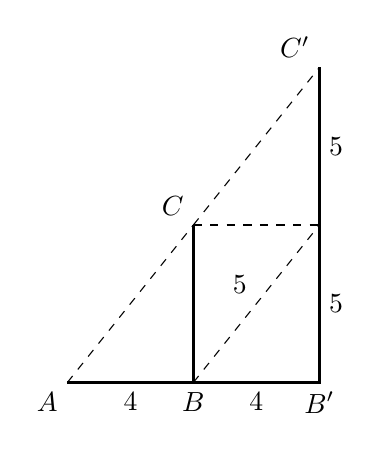
\begin{tikzpicture}
    % constants
    \def\trigwidth{1.6cm}
    \def\trigheight{2cm}
    % small triangle nodes
    \coordinate [label={below left:$A$}]   (A) at (0, 0);
    \coordinate [label={below:$B$}]  (B) at (\trigwidth, 0);
    \coordinate [label={above left:$C$}]  (C) at (\trigwidth, \trigheight);
    % large triangle nodes
    \coordinate [label={below:$B'$}] (B') at (2*\trigwidth, 0);
    \coordinate [label={above left:$C'$}] (C') at (2*\trigwidth, 2*\trigheight);
    \coordinate (B'C'mid) at (2*\trigwidth, \trigheight);
    % lengths labels
    \coordinate [label={below:$4$}] (ABmid) at (0.5*\trigwidth, 0);
    \coordinate [label={below:$4$}] (BB'mid) at (1.5*\trigwidth, 0);
    \coordinate [label={right:$5$}] (x) at (2*\trigwidth, 0.5*\trigheight);
    \coordinate [label={right:$5$}] (y) at (2*\trigwidth, 1.5*\trigheight);
    \coordinate [label={above left:$5$}] (z) at (1.5*\trigwidth, 0.5*\trigheight);
    % small triangle
    \draw [very thick] (A) -- (B) -- (C);
    \draw [dashed] (A) -- (C);
    % large triangle
    \draw [very thick] (B) -- (B') -- (C');
    \draw [dashed] (C) -- (C');
    % internal lines
    \draw [dashed] (C) -- (B'C'mid);
    \draw [dashed] (B) -- (B'C'mid);
\end{tikzpicture}
\caption{Using similar triangles to measure the height of a tree}
\end{figure}

\begin{theorem}
(Thales’ intercept theorem). Consider an arbitrary triangle $ABC$ (see figure \ref{geo:similar-triangles} below) and let $AC$  be extended to $C'$ and $AB$ to $B'$ so that $B'C'$ is parallel to $BC$. Then the lengths of the sides satisfy the relations
\[
\frac{a'}{a} = \frac{b'}{b} = \frac{c'}{c}
\textrm{~ and hence ~}
\frac{a'}{c'} = \frac{a}{c},~~
\frac{c'}{b'} = \frac{c}{b},~~
\frac{b'}{a'} = \frac{b}{a}
\]

\end{theorem}
As these proportions are also preserved when the triangle is displaced and rotated we get the following result. \textit{If corresponding angles of two triangles are equal, then corresponding sides are proportional}. Triangles having these properties are called similar (see figure below \ref{geo:similar-triangles}).
\begin{figure}[H]
\label{geo:similar-triangles}
\centering
\begin{tikzpicture}[x=0.6cm,y=0.6cm, rotate=10,every node/.style={draw}]
    % constants
    \def\aLength{3}
    \def\bLength{4}
    \def\cLength{5}
    \def\amLength{6}
    \def\bmLength{8}
    \def\cmLength{10}
    % small triangle nodes
    \coordinate [label={below left:$A$}] (A) at (0, 0);
    \coordinate [label={below:$B$}] (B) at (\cLength, 0);
    \coordinate [label={above left:$C$}] (C) at (\cLength, \aLength);
    % large triangle nodes
    \coordinate [label={below right:$B'$}] (B') at (\cmLength, 0);
    \coordinate [label={above right:$C'$}] (C') at (\cmLength, \amLength);
    % length labels
    \coordinate [label={right:$a$}] (a) at (\cLength, 0.5*\aLength);
    \coordinate [label={above:$b$}] (b) at (0.5*\bLength, 0.5*\aLength);
    \coordinate [label={below:$c$}] (c) at (0.5*\cLength, 0);
    \coordinate [label={right:$a'$}] (a') at (\cmLength, 0.5*\amLength);
    \coordinate [label={above right:$b'$}] (b') at (0.5*\bmLength, 0.5*\amLength+0.75);
    \coordinate [label={below:$c'$}] (c') at (0.5*\cmLength, -0.75);
    % angel labels

    % small triangle
    \draw [very thick] (A) -- (C) -- (B) -- (A);
    % large triangle
    \draw [dashed] (B) -- (B') -- (C') -- (C);
\end{tikzpicture}
\caption{Similar triangles $\Delta ABC$ and $\Delta AB'C'$}
\end{figure}

An important point is that the above description of Thales intercept theorem does not consitute a proof but is mearly a statement. For regerious mahtmetical proofs we will turn the master of classical geometry, Euclid.

\section{Euclidean Geometry}
Euclid is righly refered to as the "Father of Geometry". He was active in Alexandria (then part of Greece, today part of Egypt) during the reign of Ptolemy I ($323-283$ BC). His collection of books, known as the Elements is one of the most influential works in the history of mathematics.

\subsection{Euclid's definitions}
% http://aleph0.clarku.edu/~djoyce/elements/bookI/bookI.html
The Elements begins with definitions of the basic concepts: point, line, angle, circle, triangle, quadrilateral. All of which to this day contrinous to be tought to millions of school children around the world. Below is a refresher of the most important once,with commentary on their defnitions.

\begin{description}
\item [Definition 1: Point] "A point\index{point} is that which has no part" says that a point serves only as a marker of location and has no width, length, or breadth.
\begin{figure}[H]
\centering
\begin{tikzpicture}
    \coordinate [label={below left:$A$}] (A) at (0, 0);
    \coordinate [label={below right:$B$}] (B) at (2, 1);
    \fill (A) circle[radius=2pt];
    \fill (B) circle[radius=2pt];
\end{tikzpicture}
\caption{Two points $A$ and $B$}
\end{figure}

\item [Definition 2-4: Lines] Definition $2$ says "A line is breadthless length". That is a line will have one dimension, length, but it won’t have breadth. Today we use the term curve for arbitrary lines that may or may not be stright. When we speak of lines they are typically streight and continous indefinitely in either direction (Euclid defines a streight line in his fourth definition as "A straight line is a line which lies evenly with the points on itself"). Finally we call lines that starts in a point and goes on indefinitely in one direction a ray\index{ray} and a line drawn between two points in known as a segment\index{segment}.
\begin{figure}[H]
\begin{subfigure}[b]{0.2\textwidth}
    \begin{tikzpicture}
        \tkzDefPoint(0,0){A};
        \tkzDefPoint(2,1){B};
        \tkzDrawPoints(A,B)\tkzLabelPoints(A,B)
        \draw (A) to[out=-20,in=-70] (B);
    \end{tikzpicture}
    \caption{Curve}
\end{subfigure}
%
\begin{subfigure}[b]{0.3\textwidth}
    \begin{tikzpicture}
        \tkzDefPoint(0,0){A};
        \tkzDefPoint(2,1){B};
        \tkzDrawPoints(A,B)\tkzLabelPoints(A,B)
        \tkzDrawLine[add= 0.25 and 0.25](A,B);
    \end{tikzpicture}
    \caption{Line}
\end{subfigure}
%
\begin{subfigure}[b]{0.25\textwidth}
    \begin{tikzpicture}
        \tkzDefPoint(0,0){A};
        \tkzDefPoint(2,1){B};
        \tkzDrawPoints(A,B)\tkzLabelPoints(A,B)
        \tkzDrawLine[add= 0 and 0.25](A,B);
    \end{tikzpicture}
    \caption{Ray}
\end{subfigure}
%
\begin{subfigure}[b]{0.2\textwidth}
    \begin{tikzpicture}
        \tkzDefPoint(0,0){A};
        \tkzDefPoint(2,1){B};
        \tkzDrawPoints(A,B)\tkzLabelPoints(A,B)
        \tkzDrawLine[add= 0 and 0](A,B);
    \end{tikzpicture}
    \caption{Segment}
\end{subfigure}
\end{figure}

\item [Definition 2-4: Angles]
\begin{figure}[H]
\centering
\begin{tikzpicture}
  \draw
    (3,-1) coordinate (a) node[right] {a}
    -- (0,0) coordinate (b) node[left] {b}
    -- (2,2) coordinate (c) node[above right] {c}
    pic["$\alpha$", draw=orange, <->, angle eccentricity=1.2, angle radius=1cm]
    {angle=a--b--c};
\end{tikzpicture}
\end{figure}
% http://tex.stackexchange.com/questions/134615/mark-angles-with-arrows-using-tkz-euclide
% http://aleph0.clarku.edu/~djoyce/elements/bookI/defI8.html
% http://aleph0.clarku.edu/~djoyce/elements/bookI/defI9.html
% http://aleph0.clarku.edu/~djoyce/elements/bookI/defI10.html
% http://aleph0.clarku.edu/~djoyce/elements/bookI/defI11.html


\item [Circle]
\begin{figure}[H]
\centering
\begin{tikzpicture}[scale=1.5]
    \tkzDefPoint(0,0){O}
    \tkzDefPoint(1,1){B}
    \tkzDefPoint(0.55,0.45){R}
    \tkzDefPoint(1,0.99){A}
    \tkzDrawArc(O,B)(A)
    \tkzDrawLines[add = 0 and 0](O,A)
    \tkzDrawPoints(O,B)
    \tkzLabelPoints[below](O,R)
    \tkzLabelPoints[right](B)
\end{tikzpicture}
\end{figure}

\item [Triangle]
\begin{figure}[H]
\centering
\begin{tikzpicture}
  \draw
    (3,-1) coordinate (a) node[right] {a}
    -- (0,0) coordinate (b) node[left] {b}
    -- (2,2) coordinate (c) node[above right] {c}
    pic["$\alpha$", draw=orange, <->, angle eccentricity=1.2, angle radius=1cm]
    {angle=a--b--c};
\end{tikzpicture}
\end{figure}

\item [Quadrilateral]
\begin{figure}[H]
\centering
\begin{tikzpicture}
  \draw
    (3,-1) coordinate (a) node[right] {a}
    -- (0,0) coordinate (b) node[left] {b}
    -- (2,2) coordinate (c) node[above right] {c}
    pic["$\alpha$", draw=orange, <->, angle eccentricity=1.2, angle radius=1cm]
    {angle=a--b--c};
\end{tikzpicture}
\end{figure}
\end{description}

\subsection{Euclid's Postulates}
Euclid then states ten axioms (also called postulates) on which all subsequent reasoning is based. The first five posgulates are:
\begin{enumerate}
    \item Two points determine a unique straight line
    \item A straight line extends indefinitely far in either direction
    \item A circle may be drawn with any given center and any given radius
    \item All right angles are equal
    \item Given a line l ( Fig. 6–1 ) and a point P not on that line, there exists in the plane of P and l and through P one and only one line m , which does not meet the given line l .
\end{enumerate}

% TODO proof - On a given finite straight line AB to construct an equilateral triangle. A B Γ ∆ E The construction is performed by describing a circle∆centred at A and passing through B (Post. 3) and another circle E centred at B and passing through A (Post. 3). Their point of intersectionΓis then joined to A and to B (Post. 1). The distance AΓis equal to BΓand to AB, which makes the triangle equilateral.

% TODO proof Eucl. I.4, I.8, VI.2 (TODO is this thales theorem)

% TODO proof - The sum of the three angles of an arbitrary triangle ABC is equal to two right angles:

% TODO interestinf geometric things to proof
% - angles of triqngles, quadrilaterals and circles
% - area/of triangles and quadrilaterals
% - pythagoras (move proof from geometry history book)
% - Squaring the circle. Finding a square whose area is equal to that of a given rectangle
% - Doubling the cube. The problem is:find a cube whose volume is twice that of a given cube
% - Trisecting an angle.
% - Find (all) right-angled triangles with all sides (TODO proof that no more exists)

Adding four right-angled triangles with sides a and b, we arrive at and get the large square of area $(a + b)^2 = a 2 + 2ab + b 2$ . Since the areas of the four triangles add up to $2ab$, the square with area $c^2$ also has area $a^2 + b^2$.

% TODO proof - An exterior angle of a triangle is greater than either remote interior angle of the triangle.



\section{Area and perimeter}
The area of a parallelogram is $a \cdot h$, where h is the altitude of the parallelogram (Eucl. I.35). There are two ways to see this: (a) We cut off the triangle on the left and add it on the right to obtain a rectangle (Euclid’s proof, see the second figure in Fig. 1.11); (b) We cut the parallelogram parallel to AB into a large number of very slim rectangles. The area of a triangle is half the area of the parallelogram.

\subsection{Triangles}
Figure 1.2 shows a right-angled triangle (ie a triangle with one angle of 90°) with another angle denoted by the Greek letter theta θ. The sides of the a right-angled triangle are called the adjacent side (next to θ), the opposite side (opposite to θ) and the hypotenuse (opposite the right-angle).

\subsection{Circle}

\noindent The area of a circle is
\begin{equation}
A = \pi \cdot r^2
\end{equation}
the perimeter (circumference) is
\begin{equation}
C = 2\pi \cdot r
\end{equation}

\section{Classical solid geometry}
\subsection{Cube}
\subsection{Cone}
\subsection{Sphere}

\section{Trigonometry}
% TODO Missing Trigonometry
% - Pythagorean trigonometric identity
% - Unit circle

\subsection{Radians}
% TODO draw radian drawing
Degrees are often used when introducing geometry. However for more advanced  work we often meassure angles in radians. Radians equals the ratio between the length of an angle arc and its radius. As the circumference of a circle equals $2\pi r$ thus an angle of $360 deg$ equals $\frac{2\pi r}{r} = 2\pi$ radians. Radians allow us to use real numbers in the trigonometric functions, rather than degrees, which are an arbitrary angular measurement between $0-360$. The use of real numbers for measuring angels allow is essential in more advanced mathematics, calculus for example.

\section{Exercises}
\begin{ExerciseList}

% TODO
% - area calculation excericses (amount of tiles 0.25m^2 tiles needed to cover 15m^2
% - compare area and peremter of squares
% - using thales theorem

\end{ExerciseList}

\chapter{Arithmetic}\label{arit}
% TODO arithmetic missing concepts
% - Ratio (3 to 1 = 3:1 means that for each time there is 3 of one type there is 1 of another).
% -- if a and b are in ratio 5:6 means for each time there is 5 of a there is 6 of b.
% -- if asked how many of type a there are if there are 12 of b we can calculate as (5/6) * 2 = 10/12
% - inequalities http://www.mathsisfun.com/algebra/inequality.html
% - absolute value
% Commutative property of multiplication (changing the order of factors in a multiplication problem and see how it affects the product.)
% Distributive property of multiplication (decomposing the factors in multiplication problems and see how it affects the product.) (9 x 8 = 4x8 + 5x8 = 32 + 40 = 72, 12 * 5 = 6*5 + 6*5 = 30 + 30 = 60)
% Associative property of multiplication (changing the grouping of factors in multiplication problems and see how it affects the product. 2×3×7 = (2×3)×7)
% http://www.theguardian.com/science/alexs-adventures-in-numberland/2015/may/21/how-to-solve-the-maths-puzzle-for-vietnamese-eight-year-olds-that-stumped-parents-and-teachers
% - rates

% \glsentry{cube}{the cube of a number is the number multiplied by itself twice, eg 3 cubed = $3^3 = 3 × 3 × 3 = 27$.}

% \glsentry{integer}{Positive and negative whole numbers such as -34, -5, 0, 1, 17, 1021}

% \glsentry{product}{The result of multiplying together two or more numbers or things, eg the product of 4 and 5 is 20.}

%\glsentry{quotient}{The result of dividing one number by another. The quotient of 14 and 7 is 2 as 14/7 = 2.}

Numbers are an integral part of nature, a day can be split into $24$ equal parts, each of our hands has five fingers and so on. Thus even without any formal study of arithmetic humans have an elementary understanding of numbers. Arithmetic, the oldest branch of mathematics, consist of the study of numbers and the basic operations between them — addition, subtraction, multiplication and division.

\myindent The earliest formal concepts of numbers dates back to the Babylonian, Egyptian and later Greek and Romean civilizations. Here tax collectors used tablets to record the tax payments of each citizen. When tabulating the tax payments various shorthands was invented. If a citizen payed five animals a tax collector may have written \rom{1}\rom{1}\rom{1}\rom{1}\rom{1}. Each \rom{1} representing one animal. If later additional five animals where collected he may have written \rom{10} instead of \rom{1}\rom{1}\rom{1}\rom{1}\rom{1}\rom{1}\rom{1}\rom{1}\rom{1}\rom{1} as its easer to read and deal with. From these early tabulation shorthands rose the first numerical systems where it was agreed upon to let specific symbols represent a quantity. By the far the most successful of these was the, still familiar, roman symbols \rom{1}, \rom{2}, \rom{3}, \rom{4}, \rom{5}, \rom{6}, \rom{7}, \rom{8}, \rom{9} and \rom{10}. Once the numbers was established various properties of them was researched, for example the greeks discovered the primes, which book \rom{7} of Euclid's elements deals extensively with. The concept of rational (fractional) numbers was also quickly arrived at as a useful device for division, such as dividing the land belonging to a village evenly among its inhabitants for harvesting. Egyptians used the word "nfr" to denote zero balance in accounting and later during the $7th$ century AD, negative numbers were used in India to represent debts.

\myindent The use of numbers in trading and science quickly outgrew the capabilities of the early numerical systems. The romans for example had no concept of number position, that is the use of the same symbol for the different orders of magnitude (for example, the "ones place", "tens place", "hundreds place"). This lack of position required them to either come up with new symbols for ever greater numbers (for example \rom{100} for $100$ and \rom{1000} for $1000$) thus greatly increasing the complexity of the system. Or to simply keep count using the symbols they already had (for example writing $11111$ as \rom{11111}). These shortcomings eventually led to efforts of creating a new better numeral system and around $400 AD$ a new system began surfacing in India. This new system used the position of ten numbers $0-9$ to denote any possible integral value.

\section{Hindu numeral system}
The Hindu numeral system was invented between the $1st$ and $4th$ centuries by Hindu mathematicians. The system was adopted, by Persian and Arab mathematicians in the $9th$ century and from the $14th$ century on, Roman numerals began to be replaced by it; however, this process was gradual, and the use of Roman numerals continues to this day.

The main advantage of the Hindu numeral system is it use of position to denote order of magnitude thus requiring far fewer different symbols to represents numbers as well as greatly simplifying operations such as adding and subtracting those numbers. For example the number $2506$ is represented as
\[
2506 = 2 \times 1000 + 5 \times 100 + 0 \times 10 + 6 \times 1.
\]
% TODO explain addition and subtraction in this system

\section{Exponenets and logarithms}
In 1544 {Michael Stifel}\index{Michael Stifel} (1487-1567) observed that $x^2 \times x^3 = (x \times x) \times (x \times x \times x) = x \times x \times x \times x \times x = x^5$ and noted that this  result could have been arrived at quickly simply by adding the exponents $2$ and $3$ so that $x^2 \times x^3 = x^{2+3}$. Using the general exponentiation notation
\[
x^n = \underbrace{x \times \dots \times x}_n
\]
this let to the general rule that
\[
x^m \times x^n = x^{m+n}
\]
Similarly, dividing exponents $\frac{x^3}{x^2} = \frac{x \times x \times x}{x \times x} = x = x^1 = x^{3-2}$ let to the generalization that 
\[
\frac{x^m}{x^n} = x^{m-n}
\]
Early in the development of exponent notation the above rule encountered issues when the exponent of the denominator was greater than that of the numerator, as in $x^3/x^5$, where the rule would give us $x^{3-5} = x^{-2}$. However by letting $x^{-n} = 1/x^n$ we obtain $x^{3-5} = x^{-2} = 1/x^2$ which agrees with the results of dividing $x^3$ by $x^5$ directly. When $m = n$ the above rule leads $x^m/x^n = x^{m-n} = x^0$ which we must define as one. 

The use of exponents was greatly boosted by the Scottish landowner {John Napier}\index{John Napier} (1550-1617) who invented {logarithms}\index{logarithms} while searching for a way to simplify computation of large numbers. His idea was to utulize the $x^n \times x^m = x^{n+m}$ property of exponents to simplify multiplication and division as it was generally agreed that multiplication and devision was more dificult than addition and subtraction. 

% TODO describe logarithmic base
% TODO describe computation with logarithmeic tables and how they where constructed 
% log (ab) = log a + log b
% log (a/b) = log a - log b
%log a^n = n log a,

\section{Decimal numbers}

using exponents we can rewrite $2506$ as
\[
2506 = 2 \times 10^3 + 5 \times 10^2 + 0 \times 10^1 + 6 \times 10^0.
\]
further taking advantage that $x^{-n} = \frac{1}{x^n}$ we see that $0.1 = \frac{1}{10} = 1 \times 10^{-1}$ and $0.02 = \frac{2}{100} = 2 \times 10^{-2}$ using this knowledge we can write decimal numbers as sums of integers and fractions, for example
\[
5678.12 = 5 \times 10^3 + 6 \times 10^2 + 7 \times 10^1 + 8 \times 10^0 + 1 \times
10^{-1} + 2 \times 10^{-2}
\]
Generally we represent a number with $n$ integer digits $a_0 \cdots a_n$ and $m$ decimal digits $b_0 \cdots b_m$ as
% TODO as
\[
a_0 \cdots a_n.b_0 \cdots b_m = a0 = a^0 \times 10^n + \cdots + a^n \times 10^0 . b^0 \times 10^{-1} + \cdots + b^m \times 10^{-m}
\]
the class of numbers that can be written in this way is called {algebraic numbers}\index{Algebraic numbers}. From the above formula we also see the well known fact that when a decimal number is multiplied by $10$, every figure moves one place to the left
\begin{align*}
1.25 \times 10 =& (1 \times 10^0 + 2 \times 10^{-1} + 5 \times 10^{-2}) \times 10 \\
               =& 1 \times 10^1 + 2 \times 10^0 + 5 \times 10^{-1}                \\
               =& 12.5                                                            \\
\end{align*}
and when you divide by $10$, every figure moves one place to the right i.e
\begin{align*}
\frac{1.25}{10} =& 1.25 \times 10^{-1}                                                  \\
                =& (1 \times 10^0 + 2 \times 10^{-1} + 5 \times 10^{-2}) \times 10^{-1} \\
                =& 1 \times 10^{-1} + 2 \times 10^{-2} + 5 \times 10^{-3}               \\
                =& 0.125                                                                \\
\end{align*}

\subsection{General Numeral systems}
% TODO move to later number section
% TODO binary numbers http://www.wildbunny.co.uk/blog/2012/11/07/understanding-binary/
As time passed positional numbers systems was generalized such that the digits ($0-9$ in the decimal system) could be changed to accomedate different purposes. For example electric current can be in only two states on (power is flowing) or off (no power). Thus in cumputers its convinient to represent numbers using only two digits $0$ and $1$. To represent higher numbers multiple wires in either on or off states can be used for example if we have $4$ wires and all are on we can represent
\[
  1 \times 2^0 + 1 \times 2^1 + 1 \times 2^2 + 1 \times 2^3 = 1 + 2 + 4 + 8 = 15
\]
If all wires are off we have
\[
  0 \times 2^0 + 0 \times 2^1 + 0 \times 2^2 + 0 \times 2^3 = 0 + 0 + 0 + 0 = 0
\]
if the first and last are on we have

Thus with a four digit number in a binary number system we can represent the integers $0-15$ or $2^4$ different values. 

The generalized binary number looks like this where each bit bits, short for binary digits, is either 0 or 1.

% TODO generalized base conversion
A simple way to convert decimal to binary is the even/odd -divide by two algorithm. This algorithm uses the following steps: If the number is even, emit a 0. If the number is odd, emit a 1. Divide the number by 2 and throw away any fractional component or remainder. If the quotient is 0, the algorithm is complete. If the quotient is not 0 and is odd, insert a 1 before the current string; if the number is even, prefix your binary string with 0. Go back to step 2 and repeat.

binary numbers are very verbose you need 8 bits to represent the number 202. Although we can convert between decimal and binary, the conversion is not a trivial task and since computers only understands binary at their corr, such a conversion would have to happen allot. The hexadecimal (base 16) numbering system solves many of the problems inherent in the binary system. Hexadecimal numbers offer the two features we're looking for: They're very compact, and it's simple to convert them to binary and vice versa. 

Each hexadecimal digit can represent one of 16 values between 0 and 1510. Because there are only 10 decimal digits, we need to invent 6 additional digits to represent the values in the range 1010..1510. Rather than create new symbols for these digits, we'll use the letters A..F. 

Ag first base 16 may seam hard to calculatr with but remebering $(a^m)^n = a^(n \times m)$ gives us that $16^2 = (2^4)^2 = 2^8 = 256$

% Decimal Binary  Hexadecimal  
% 0       0000  $0  
% 1 0001  $1  
% 2 0010  $2  
% 3 0011  $3  
% 4 0100  $4  
% 5 0101  $5  
% 6 0110  $6  
% 7 0111  $7  
% 8 1000  $8  
% 9 1001  $9  
% 10 1010  $A  
% 11 1011  $B  
% 12 1100  $C  
% 13 1101  $D  
% 14 1110  $E  
% 15 1111  $F  

To convert a hexadecimal number into a binary number, simply substitute the corresponding 4 bits for each hexadecimal digit in the number. For example, to convert ABCD into a binary value, simply convert each hexadecimal digit according to Table 2-1, as shown here: A  B  C  D  Hexadecimal  1010  1011  1100  1101  Binary  To convert a binary number into hexadecimal format is almost as easy. The first step is to pad the binary number with zeros to make sure that there is a multiple of 4 bits in the number. For example, given the binary number $1011001010$, the first step would be to add 2 bits to the left of the number so that it contains 12 bits. The converted binary value is $001011001010$. The next step is to separate the binary value into groups of 4 bits, for example, $0010\_1100\_1010$. Finally, look up these binary values in the table above.

Note that shifting a value to the left is the same thing as multiplying it by its radix. For example, shifting a decimal number one position to the left (adding a 0 to the right of the number) effectively multiplies it by 10 (the radix): 1234 shl 1 = 12340 (shl 1 means shift one digit position to the left.) Because the radix of a binary number is 2, shifting it left multiplies it by 2. If you shift a binary value to the left twice, you multiply it by 2 twice (that is, you multiply it by 4). If you shift a binary value to the left three times, you multiply it by 8 (2*2*2). In general, if you shift a value to the left n times, you multiply that value by 2n.

\myindent In the generalized positional number system we use the \index{base} (or \index{radix}) to represent the different symbols available to each digit within that system. For example, the decimal system has a radix of $10$, that is any diget in a number can have values $0-9$. In contrary computers work using electronic circuits and thus digets are represented with radix $2$. Other commonly used number systems are hexadecimal wich uses radix $16$ with digets represented with the numbers $0-9$ and letters $A-F$. Generally we have

\subsection{Decimal representation}
\[
(a_{n}a_{n-1} \cdots a_{1}a_{0} . c_{1}c_{2} \cdots c_{m-1}c_{m}) =
    \sum_{k=0}^{n}a_{k}b^{k} + \sum_{k=1}^{m}c_{k}b^{-k}
\]
The numbers $b^{k}$ and $b_{k}$ are the weights of the corresponding digits. The position $k$ is the logarithm of the corresponding weight $w$, that is $k = \log_{b} w = \log_{b} b^k$

% TODO repeating decimals 0.77777 = 7/9

For example to write $1/3$ in base $16$ we get
% TODO http://en.wikipedia.org/wiki/Hexadecimal#Conversion

\subsection{Conversion between systems}
% - Number bases (convert 1/2 from base 10 base 6)

\subsection{Scientific notation}
Scientific notation is a way of writing numbers that are too big or too small to be conveniently written in decimal form. In scientific notation all numbers are written in the form
\[
a \times 10^b
\]
where the exponent $b$ is chosen so its absolute value is at least one but less than ten ($1 \leq |a| < 10$). Thus $350$ is written as $3.5×10^2$. The following table are examples of scientific notation:
\begin{figure}[H]
\centering
\begin{tabular}{|l|l|l|l|}
\hline
\textbf{Decimal notation}   & \textbf{Scientific notation} \\ \hline
2                           & $2 \times 10^0$              \\ \hline
300                         & $3 \times 10^2$              \\ \hline
4,321.768                   & $4,321768 \times 10^3$       \\ \hline
−53,000                     & $−5,3 \times 10^4$           \\ \hline
6,720.000.000	           & $6,72 \times 10^9$           \\ \hline
0.2	                        & $2 \times 10^{−1}$           \\ \hline
0,000.000.007.51	           & $7,51 \times 10^{−9}$        \\ \hline
\end{tabular}
\end{figure}
This form allows easy comparison of numbers, as the exponent b gives the number's order of magnitude. For example, the order of magnitude of $1500$ is $3$, since $1500$ may be written as $1.5 × 10^3$.

\subsection{Rounding}
Rounding a number means replacing it by another that is approximately equal but has a shorter or simpler representation. The procedure is as follows. \textbf{Pick the number to round to as the last digit to keep. Leave it the same if the next digit is less than 5 or increase it by 1 if the next digit is 5 or more. Finally turn all following digets into zeros}. The following examples demonstrate the rounding procedure:

\begin{description}
\item [Round to the nearest hundred] $838.274$ is $800$ as $3 < 5$
\item [Round to the nearest ten] $838.274$ is $840$ as $8 > 5$
\item [Round to the nearest one] $838.274$ is $838$ as $2 < 5$
\item [Round to the nearest tenth] $838.274$ is $838.3$ as $7 > 5$
\item [Round to the nearest hundredth] $838.274$ is $838.27$ as $4 < 5$
\end{description}

Besides the standard rounding mentioned above two other methods called floor and ceiling which maps a real number to the largest previous or the smallest following integer, respectively. More precisely, $floor(x) = \lfloor x \rfloor$ is the largest integer not greater than $x$ and $ceiling(x) =  \lceil x \rceil$ is the smallest integer not less than $x$.
\begin{figure}[H]
\centering
\begin{tabular}{|l|l|l|l|}
\hline
\textbf{Value}  & \textbf{Floor} & \textbf{Ceiling} & \textbf{Fractional part} \\ \hline
2.4	            & 2	            & 3	              & 0.4                      \\ \hline
2.9	            & 2	            & 3	              & 0.9                      \\ \hline
-2.7	            & -3	            & -2	              & 0.3                      \\ \hline
-2	            & -2	            & -2	              & 0                        \\ \hline
\end{tabular}
\end{figure}

\subsection{Significant figures}
The significant figures of a number are those digits that carry meaning contributing to its precision. The procedure for identifying significant figures is as follows
\begin{enumerate}
\item Identify the non-zero digits and any zeros between them. These are all significant.
\item Leading zeros are not significant.
\item If its a decimal, then trailing zeros are significant.
\end{enumerate}

\newpage
\section{Addition}
% TODO missing addition concepts
% - describe adding decimals
Addition represents the operation of adding objects to a collection. For example, $2+3$ can be though of as if you have $2$ apples and someone give you $3$ more, then you have $5$ apples in total. Assuming $b$ is positive then on a number line $a+b$ represents starting on number $a$ and moving $b$ places to the right. Similar if $b$ is negative then $a+b$ represents starting on number $a$ and moving $b$ places to the left. Unlike subtraction the addition operations is both commutative (that is $a + b = b + a$) and associative (that is $a + (b + c) = (a + b) + c$)

\begin{description}
\item [Adding integers] We add integers by adding the ones, tens,hundreds etc. in each number individually, starting from the right. If the result of addition is above $10$ then we subtract $10$ from the result and add one (known as a carry) to the next group to be added. For example
\begin{figure}[H]
\centering
\opadd{143}{89}
\end{figure}
That is we add $3+9=12$ as the result is above $10$ we subtract $10$ from it and add one tenth to the tenths place. In the tenth place we now add $1+3+8=12$ which again is above $10$, so we subtract $10$ from it and add $1$ to the hundreds place (ten tens being one hundred) and so finally we add $1+1$ in the hundreds place.

To understand why this procedure works consider that the number $143 = 100 + 40 + 3$ and $89 = 80 + 9$ so we can do
\[
\begin{align}
143 + 89 &= (100 + 40 + 3) + (80 + 9) \\
         &= 100 + (40+80) + (3+9)     \\
         &= 100 + (40+80) + 12        \\
         &= 100 + (10+40+80) + 2      \\
         &= 100 + 130 + 2             \\
         &= (100 + 100) + 30 + 2      \\
         &= 232
\end{align}
\]
\item [Adding decimals] We add decimals semilar to integers by starting
from the rightmost decimal.
\begin{figure}[H]
\centering
\opadd{9.087}{15.924}
\end{figure}
\end{description}

\section{Subtraction}
Subtraction represents the operation of removing objects from a collection. For example, $5-2$ can be though of as if you have $5$ apples and take $2$ away, then you have $3$ apples left. Assuming $b$ is positive then on a number line $a-b$ represents starting on number $a$ and moving $b$ places to the left. Similar if $b$ is negative then $a-b$ represents starting on number $a$ and moving $b$ places to the right.

Subtraction is not commutative, that is $a - b \neq b - a$ instead we can reverse the subtraction order by $a - b = -(b - a) = -b + a$. Further subtraction is not associative so $a  - (b - c) \neq (a - b) - c$ instead it holds $a - b - c = a - (b + c)$ and $a - b - c - d = a - (b + c + d)$ and so on.
\begin{description}
\item [Subtracting integers] We subtract numbers by subtracting each
ones, tens, hundreds etc. individually, starting from the right, if the
subtraction yields a result less than zero then we borrow ten from the
number to the left by decreasing its value by one:
\begin{figure}[H]
\centering
\opsub{133}{89}
\end{figure}
\item [Subtracting decimals]
% TODO subtracting decimals
\end{description}

\section{Multiplication}
Multiplication of two whole numbers is equivalent to the addition of one of them with itself as many times as the value of the other one; for example, $3 \cdot 4$ can be calculated by adding $4$ to itself $3$ times:
\[
3 \cdot 4 = 4 + 4 + 4 = 12
\]
it can also be calculated by adding $4$ copies of $3$ together:
\[
3 \cdot 4 = 3 + 3 + 3 + 3 = 12
\]
Formally we say that multiplication is both commutative (i.e. the order in which two numbers are multiplied does not matter $a \cdot b = b \cdot a$) and associative $a \cdot (b \cdot c) = (a \cdot b) \cdot c$. Multiplication has other important properties:
\begin{description}
\item [Distributive property] Holds with respect to multiplication over addition. This identity is of prime importance in simplifying algebraic expressions: $x\cdot(y + z) = x\cdot y + x\cdot z$
\item [Identity element] The multiplicative identity is $1$; anything multiplied by one is itself. This is known as the identity property: $x\cdot 1 = x$
\item [Zero element] Any number multiplied by zero is zero. This is known as the zero property of multiplication: $x\cdot  0 = 0$
\end{description}

% TODO missing multiplication areas
% - explain operations of single and multi diget
% - explain meaning of multiplying negative numbers
% - explain techniques for muktiplication
\begin{description}
\item [Multiplying integers] We multiply integers by multiplying the ones, tens, hundreds etc. in each number individually, starting from the right. If the result of multiplication is above $10$ we subtract $10$ from the result and add one (known as a carry) to the next group to be multiplied. For example
\begin{figure}[H]
\centering
\opmul[displayintermediary=None]{142}{3}
\end{figure}

That is we first multiply $3 \cdot 2 = 6$ in the ones place, then in the tenth place we multiply $3 \cdot 4 = 12$ which is above $10$, so we subtract $10$ from it and add $1$ to the hundreds place and so finally we multiply $3 \cdot 1 = 3$ and add the carry of $1$ to it in order to get $4$ in the hundreds place.

To understand why this procedure works consider that the number $142 = 100 + 40 + 2$ so really we have
\[
\begin{align}
143 \cdot 3 &= (100 + 40 + 2) \cdot 3  \\
            &= (100 \cdot 3) + (40 \cdot 3) + (2 \cdot 3)  \\
            &= (100 \cdot 3) + (10 \cdot 4 \cdot 3) + 6  \\
            &= (100 \cdot 3) + (10 \cdot 12) + 6  \\
            &= (100 \cdot 3) + (100 + 20) + 6  \\
            &= (100 \cdot 4) + 20 + 6  \\
            &= 426
\end{align}
\]

\item [Multiplying decimals] To multiply decimals convert them into integers, multiply them and then convert the result back to a decimal i.e.
\begin{itemize}
\item $8 * 0.8 = 8 * \frac{8}{10} = \frac{64}{10} = 6.4$
\item $2.91 * 3.2 = \frac{291}{100} * \frac{32}{10} = \frac{291 * 32}{1000} =
\frac{9312}{1000} = 9.312$
\end{itemize}
\end{description}

\section{Fractions}
In the fraction $3/4$, the numerator $3$ (also known as the dividend) tells us that the fraction represents $3$ equal parts, and the denominator $4$ (also known as the divisor) tells us that $4$ parts make up a whole. The fraction $5/4$ equally tells us that $4/4$ makes up a whole and we have an extra $1/4$ part left.
% TODO define remainder and quotient
\begin{description}
% TODO explain why these works
\item [Equal fractions] Fractions have the same value when they represent the
same parts of a hole e.g. $\frac{a}{b} = \frac{c}{d}$ if and only if
$a \cdot d = b \dot c$.
\item [Ordering fractions] When both denominators are positive
$\frac{a}{b} < \frac{c}{d}$ if and only if $ad < bc$. If either denominator is
negative convert them into postive numbers by negating the numerator.
\item [Additive inverse] $-\left(\frac{a}{b}\right) = \frac{-a}{b} = \frac{a}{-b}$
\item [Multiplicative inverse] $\left(\frac{a}{b}\right)^{-1} = \frac{b}{a}$
\item [Simplifying Fractions] (TODO examples 78/52
\item [Adding fractions] $\frac{a}{b} + \frac{c}{d} = \frac{a*d + b*c}{b*d}$
\item [Subtracting fractions] $\frac{a}{b} - \frac{c}{d} = \frac{a*d - c*c}{b*d}$
\item [Multiplying fractions] $\frac{a}{b} * \frac{c}{d} = \frac{a*b}{c*d}$
\item [Dividing fractions] Division is equivalent to multiplying by the
reciprocal of the divisor fraction: $\frac{a}{b}/\frac{c}{d} =
\frac{a}{b} \cdot \frac{d}{c}$
\item [Exponentiation to integer power] If $n$ is a non-negative integer, then
$\left(\frac{a}{b}\right)^{n} = \frac{a^n}{b^n}$ and if $a \neq 0$ then
$\left(\frac{a}{b}\right)^{-n} = \frac{1}{\left(\frac{a}{b}\right)^n} =
\frac{1}{\frac{a^n}{b^n}} =\frac{b^n}{a^n}$.
\item [Converting decimals to fractions] Place the decimal in the numerator
and one in the denominator and multiply both with multiples of ten until the
decimal point disapears e.g. $0.024 = 0.024/1 = 0.24/10 = 2.4/100 = 24/1000$
\end{description}

\subsection{Mixed numbers}
Improper fractions such as $5/4$, where the numerator is larger than the denominator, are commonly represented as a combination of a whole number and a proper fraction called a mixed number e.g. $5/4 = 1\frac{1}{4}$.
\begin{description}
\item [Converting fractions to mixed numbers] Convert the numerator to a sum where the first part can be divided by the denominator and the last part has a lower value than the denominator e.g. $\frac{64}{5} = \frac{60 + 4}{5} = \frac{60}{5} + \frac{4}{5} = 12 \frac{4}{5}$
\item [Converting mixed numbers to fractions] Multiply the leading integer with the denominator and add it to the numerator e.g. $12 \frac{2}{3} = \frac{3 * 12 + 2}{3} = \frac{38}{3}$
\item [Adding and subtracting mixed numbers] A mixed number $a \frac{b}{c}$ is a short hand for $a + \frac{b}{c}$ so to add or subtract mixed numbers perform the operation step wise on the integer and fractional part of the numbers e.g. $6\frac{6}{12} - 3\frac{3}{5} = 6 + \frac{6}{12} - 3 - \frac{3}{5} = 2\frac{9}{10}$.
\item [Multiplying mixed numbers] Convert the mixed number to a fraction and multiply these e.g. $1\frac{1}{4} * 4 = \frac{20}{4} = 5$
\end{description}


\section{Division}
% TODO missing division
% - using  prime factorisation to simplify numbers (see number theory)
% - factors
% - GCD and LCM
% - explain why division algo works
% - division commutativity and associative
\begin{description}
\item [Dividing improper fractions] Division is really counting the number of repeated subtractions of the divisor into the dividend e.g. $3024/42 = 72$ as shown below
\newline
\[
\begin{array}{*{6}{>{\hfill}m{7mm}}}
 &
     &
         0&
             0&
                 7&
                     2\\\cline{3-6}
4&
  2\big)&
        3&
             0&
                 2&
                     4\\\cline{1-2}
 &
     &
        2&
            9&
                4&
                     \\\cline{3-5}
 &
     &
         &
             &
                8&
                     4\\
 &
     &
         &
             &
                 8&
                     4\\\cline{5-6}
\end{array}
\]
\item [Dividing proper fractions] As proper fractions always represent values parts less than 1 whole we know the result must be a decimal beginning with 0.
\[
\begin{array}{*{7}{>{\hfill}m{7mm}}}
 &
     &
         &
           0,&
                7&
                    0&
                        3\\\cline{3-7}
2&
  7\big)&
        1&
           9,&
                0&
                    0&
                        0\\\cline{1-2}
 &
     &
        1&
            8&
                9&
                     &
                         \\\cline{3-5}
 &
     &
         &
             &
                1&
                    0&
                        \\
 &
     &
         &
             &
                 &
                     0&
                        \\\cline{5-7}
 &
     &
         &
             &
                 1&
                     0&
                         0\\
 &
     &
         &
             &
                 &
                     8&
                         1\\\cline{6-7}
 &
     &
         &
             &
                 &
                     1&
                         9\\
\end{array}
\]
\item [Dividing decimals] To divide decimals first convert the denominator into a integer then divide the resulting fraction as shown above e.g. $3.3534/0.81 = 335.34/81$
\[
\begin{array}{*{7}{>{\hfill}m{7mm}}}
 &
     &
        0&
            0&
                4,&
                    1&
                        4\\\cline{3-7}
8&
  1\big)&
        3&
            3&
                5,&
                    3&
                        4\\\cline{1-2}
 &
     &
        3&
            2&
                4&
                     &
                         \\\cline{3-5}
 &
     &
         &
             1&
                1&
                    3&
                        \\
 &
     &
         &
             &
                 8&
                     1&
                        \\\cline{5-7}
 &
     &
         &
             &
                 3&
                     2&
                         4\\
 &
     &
         &
             &
                 3&
                     2&
                         4\\\cline{6-7}
\end{array}
\]

\end{description}

\subsection{Divisibility tests}
% TODO proove these
The following rules can test numbers for divisibility
\begin{description}
\item [Divisible by $2$] if the last didget is divisible by $2$.
\item [Divisible by $3$] if the sum of the digits is divisible by $3$.
\item [Divisible by $4$] if the number formed by the last two digits is
divisible by $4$.
\item [Divisible by $5$] if the last digit is either $0$ or $5$.
\item [Divisible by $6$] if divisible by $2$ and $3$.
\item [Divisible by $9$] if the sum of the digits is divisible by $9$.
\item [Divisible by $10$] if the last digit is $0$.
\end{description}

\subsection{Remainder}
The remainder from the division $a/b$ is represented mathematically as $a \textrm{mod} b$, for example $9/2 = 4$ and $9 mod 2 = 1$. In general to the find the result of $a \textrm{mod} b$ we follow these steps:
\begin{enumerate}
\item Construct a clock with size $b$
\item Start at 0 and move around the clock $a$ steps (If the number is positive we step clockwise, if it's negative we step counter-clockwise).
\item Wherever we land is our solution.
\end{enumerate}
For example $7 mod 2 = 1$ since we can make a clock with numbers $0,1$ then start at $0$ and go through $7$ numbers in a clockwise sequence $1,0,1,0,1,0,1$. Similar $-5 mod 3 = 1$ since we make a clock with numbers $0,1,2$ then start at $0$ and go through $5$ numbers in counter-clockwise sequence  $2,1,0,2,1$

\section{Percents}
% TODO percents missing concepts
% - relationship between percents, fractions and divisions (100 * 1.05 = 105, 100/1.05 = ??
% - pie costs 11 price drops 45 how much do you save (11 * 0.45 = what you save, 11 * 0.55 = what it will cost)
% - wholesale price and markup (explain concepts)


\section{Exponents and roots}\label{arit:exp}
If we multiply 3 by itself 4 times we get
\[
3 \cdot 3 \cdot 3 \cdot 3 = 81
\]
A more concise way of writing this is to say
\[
3^4 = 81
\]
where 3 is the base and the superscript 4 is called the power or exponent.

% TODO compare list of rules with that from math picture taken

\begin{description}
\item [Squares $b^2$] means $b \cdot b$ and is read \emph{b squared} because $b^2$ is the area of a square whose side has length $b$.
\item [Cubes $b^3$] means $b \cdot b \cdot b$ and is read \emph{b cube} because $b^3$ is the volume of a cube whose side has length $b$.
\item [Powers of $10$] If the power is positive the result is one followed by as many zeros as the number in the exponent $10^7 = 10000000$. If the exponent is negative we have as many zeroes as the exponent followed by one with the first zero being before the comma the rest after $10^+7 = 0.0000001$
\item [Negative powers] $a^{-n} = \frac{1}{a^n}$
\item [Products of powers] $a^n \cdot a^m = a^{n+m}$ this can be seen as $5^3 \cdot 5^2 = (5 \cdot 5 \cdot 5) \cdot (5 \cdot 5)= 5^5$
\item [Products of unlike powers] $a^n \cdot b^n = (a \cdot b)^n$ this can be seen as $(2 \cdot 2 \cdot 2) \cdot (3 \cdot 3 \cdot 3) = (2 \cdot 3) \cdot (2 \cdot 3) \cdot (2 \cdot 3) = (2 \cdot 3)^3$
\item [Fractions of powers] $\frac{a^n}{a^m} = a^{n-m}$ this can be seen as $\frac{5^3}{5^2} = \frac{5 \cdot 5 \cdot 5}{5 \cdot 5} = 5^1$
\item [Powers of fractions] $\left(\frac{a}{b}\right)^n = \frac{a^n}{b^n}$ this can be seen as $\left(\frac{2}{3}\right)^3 = \frac{2}{3} \cdot \frac{2}{3} \cdot \frac{2}{3} = \frac{2^3}{3^3}$
\item [Powers of powers] $(a^m)^n = a^{(m \cdot n)}$ this can be seen as $(5^2)^3 = 5^2 \cdot 5^2 \cdot 5^2 = 5^{6}$
\item [Fractional powers] $a^{\frac{x}{y}} = (a^{\frac{1}{y}})^x$. This can be related to roots since $\sqrt{a} \cdot \sqrt{a} = a$ can be satisfied as $a^{x} \cdot a^{x} = a^{x+x} = a^{1}$ only when $x = 1/2$. That is $\sqrt{a} = a^{1/2}$. Generally we have $\sqrt[n]{a} = a^{1/n}$.
\item [Simplifying radicals] Radicals such as $\sqrt{32}$ are simplified by rewriting them to lower terms using the above rules e.g. $3\sqrt{8} - 6\sqrt{32} = 3\sqrt{4}\sqrt{2} - 6\sqrt{16}\sqrt{2} = 6\sqrt{2} - 24\sqrt{2} = -18\sqrt{2}$. Often it can be constructive to rewrite radicals using their prime factorization e.g. $\sqrt[3]{81} = \sqrt[3]{9 \cdot 9} = \sqrt[3]{3 \cdot 3 \cdot 3 \cdot 3} = 3\sqrt[3]{3}$
\end{description}

\subsection{Estimating roots}
\begin{description}
\item [Square roots]
% TODO long hand square root algorithms
% - http://xlinux.nist.gov/dads/HTML/squareRoot.html
% - http://mathforum.org/library/drmath/view/52610.html
% - http://www.embedded.com/electronics-blogs/programmer-s-toolbox/4219659/Integer-Square-Roots
\item [Cube roots] find the prime factors and see if any come three times. For example $\sqrt[3]{3430}$ is divisible by $10$ and there for have $5$ and $2$ as prime factors, $343 = 7^3$ so we have $\sqrt[3]{3430} = \sqrt[3]{2 \cdot 5 \cdot 7 \cdot 7 \cdot 7} = 7 \cdot \sqrt[3]{10}$
\end{description}

\subsection{Scientific notation}
When adding and subtracting two numbers in scientific notation, we must adjust the two values so that their exponents are the same. For example, when adding 1.23e1 and 4.56e0, we must adjust the values so they have the same exponent. One way to do this is to convert 4.56e0 to 0.456e1 and then add. This produces 1.686e1.

\section{Order of operators}\label{arit:order}
The order of arithmetic operators is as follows
\begin{enumerate}
\item Parentheses and exponents
\item Multiplication and division
\item Addition and subtraction
When multiple operations exists on the same level you do the one that it closest on the left, for example
\[
2-10+8-(-2)+(-10) = 2 - 10 + 8 + 2 - 10 = (2 - 10 + 8) + 2 - 10 = (-8 + 8) + 2 - 10 = 0 + 2 - 10 = -8
\]
\end{enumerate}

\section{Exercises}
%% EXCERCISES
% [Addition]
% - Single, multi and decimal
% [Multiplication]
% - Single, multi and decimal
% [Subtraction]
% - Single, multi and decimal
% [Division]
% - Single, multi and decimal
% 144.95/65
% [Modular arithmetic]
% - Dorothy gives a piece of candy to each of her friends in the following order and then starts over from the beginning: the Scarecrow, the Tinman, the Cowardly Lion, and Toto. Who gets the twenty-fifth piece of candy? (the Scarecrow gets it as we can finish 6 cycles of handing out candy and then begin in the first person in the group again)
% - Vincent van Gogh is making one-color versions of all his paintings. He uses the colors in the following order and then starts over from the beginning: red, blue, pink, green, and purple. What color is Painting 31 ? (Answer: red)
% [Scientific notation]
% - Express this quotient in scientific notation: \frac{7.0×10^{−4}}{5.320×10^{−2}
% - The volume of the Earth is 1.1⋅10^21 cubic meters. The volume of the sun is 1.4⋅10^27 cubic meters. How many Earths could fit inside the sun?
% - A strainbif bqcferia triples every hour,mif fhere initially ia 200bqcteria how many are fhere afger four hours (ans after one hour there are 3*200 after two there are 3*3*200 after four ghere are 3^4*200)

\begin{ExerciseList}

\Exercise Reduce the following fractions
\Question $88/72$
\Question $\frac{2}{\frac{4}{5}}$
\Question $\frac{\frac{-7}{2}}{\frac{4}{9}}$
\Answer Canceling out common terms we get
\begin{enumerate}
\item\myindent $88/72 = (11*8)/(9*8) = 11/9$.
\item\myindent $\frac{2}{\frac{4}{5}} = 2 \cdot \frac{5}{4} = \frac{10}{4} = \frac{5}{2}$
\item\myindent $\frac{\frac{-7}{2}}{\frac{4}{9}} = \frac{-7}{-2} \cdot \frac{9}{4} = \frac{63}{8}$
\end{enumerate}

\Exercise If it takes 36 minutes for $5$ people to paint $9$ walls. How many minutes does it take $10$ people to paint $7$ walls?
\Answer $36/9$ is the time it takes for $5$ people to paint one wall, therefor $5 * 36/9$ is the time it takes for one person to paint one wall. Thus it will take $7 * ((5 * 36)/9) = 140$ for one person to paint $7$ walls and therefor $140/10 = 14$ minutes for $10$ people

\Exercise Philip is going on a 4000-kilometer road trip with three friends. The car consumes $6$ liters of gas per $100$ kilometers, and gas costs $1.50$ per liter. If Philip and his friends want to split the cost of gas evenly, how much should they each pay?.
\Answer The car will spend $4000/100 * 6 = 240$ liters of gas at a price of $240 * 1.5 = 360$, as there are four people in the car the cost per person becomes $360/4 = 90$.

% TODO add to Solvr arithmetic tests
\Exercise What is the value of
\Question $7 + 7/7 + 7 \cdot 7 - 7$
\Question $6 -1 \cdot 0 + 2/2$
\Question $-2 + (-3) + 4 - (-3) - 5$
\Question $3 + (-4) - 8 - (-1) - 1$
\Answer Using the PEMDAS meme (parentheses, exponents, multiplication,
division, addition, subtraction) listed in \ref{arit:order} we get:
\begin{enumerate}
 \item\myindent $7 + 7/7 + 7 cdot 7 - 7 = 7 + (7/7) + (7 \cdot 7) - 7 = 50$.
 \item\myindent $6 - 1 \cdot 0 + 2/2 = 6 + -1 \cdot 0 + 2/2 = 6 + 0 + 2/2 = 7$
 \item\myindent $-2 + (-3) + 4 - (-3) - 5 = -2 - 3 + 4 + 3 - 5 = -5 + 7 - 5 = -3$
 \item\myindent $3 + (-4) - 8 - (-1) - 1 = 3 - 4 - 8 + 1 - 1 = -1 - 8 $
\end{enumerate}

\Exercise Reduce the following
\Question Rewrite $\frac{4^6}{4^{-4}}$ in the form $4^n$
\Question Rewrite $(5^{-12})^{-9}$ in the form $5^n$
\Question Rewrite $((5^{-10})(9^9))^7$ in the form $5^n \cdot 9^m$
\Question Rewrite $\sqrt{11} + \sqrt{44} + \sqrt{99}$ in the form $n \cdot \sqrt{m}$
\Answer Using the exponent rules from \ref{arit:exp} we get
\begin{enumerate}
\item\myindent $\frac{4^6}{4^{-4}} = 4^{6 - -4} = 4^{10}$
\item\myindent $(5^{-12})^{-9} = 5^{108}$
\item\myindent $((5^{-10})(9^9))^7 = 5^{-70} \cdot 9^{63}$
\item\myindent $\sqrt{11} + \sqrt{44} + \sqrt{99} =
                \sqrt{11} + \sqrt{4 \cdot 11} + \sqrt{9 \cdot 11} = 6\sqrt{11}$
\end{enumerate}
\end{ExerciseList}

\chapter{Basic algebra}\label{alg}
% TODO algebra missing concepts
% - solving equations (do same things at both sides)
% - Systems of equations
%  - substitution -b - a and a + b = -1
% - dependent and independent variables
% - equivalent forms of expressions
% - adding and subtracting polynomials
% - linear binomials (what does linear mean in this context)
% - linear equations
% - mononomial
% - add function examples from think like a mathematician
% - have five of each exercise type
% - Linear equations and inequalities
% - Graphing lines and slope
% - System of equations
% - Expressions and equations with exponens
% - Quadratics and polynomials
% - Equations and geometry
% - long multiplicafion for polynomials
%
%      x + 4}
%      x + 3
%-----------
%     3x +12
% x^2+4x
%-----------
% x^2+7x +12
%
% axes (left-right) and (up-down)
% ordered pairs
% Term, product, factor, coefficient 
% Fx.  (a+b+c+d)(e+f+g+h) has two factors each consisting of four terms

% the study of numbers and its extensions to algebra arose out of the very practical problems of keeping track of property, trading, taxation, and the like,
% - solve quadratics by factoring 
% - - (x^2 + 12x + 36 = (x+6)(x+6) so x=-6
% - - (4x^2 + 36x + 72) = (2x+6)(2x+12) = 4x^2 + 24x + 12x + 72 (72 = 8*9 = 2*4 * 3*3 = 6*12)
% - - (2x+6 = 0 x=-3) og (2x + 12 = 0 x=-6)
%
% - The speed of sound in an iron rod is 16,850 ft/sec, and the speed in air is 1100 ft/sec. If a sound originating at one end of the rod is heard one second sooner through the rod than through the air, how long is the rod?
% - 4.  The population of town A is 10,000 and is increasing by 600 each year. The population of town B is 20,000 and is increasing by 400 each year. After how many years will the two towns have the same population?
% 2.  Find the roots of each of the equations in Exercise 1 by forming a new equation whose roots are “larger” than those of the original equation by one- half the coefficient of x
% 
% move proof of general second degree equation from "math for non-math" (If we divide this equation by a, we obtain x 2 + ( b / a ) x + ( c / a ) = 0. This equation is now of the same form as (28) , where p = b / a and q = c / a .)
%
% Ars Magna , the first major book on algebra in modern times. After refusing to divulge the method, Tartaglia finally acquiesced, but asked Cardan to keep it secret. However, Cardan wished his book to be as important as possible and so published the method, though acknowledging that it was Tartaglia’s. From this book, which appeared in 1545, the mathematical world learned how to solve third- degree equations. In this same book Cardan also published a method of solving fourth- degree equations discovered by one of his own pupils, Lodovico Ferrari
%
% - a young Norwegian mathematician, Niels Henrik Abel (1802–1829), showed at the age of 22 that fifth- degree equations could not be solved by the processes of algebra. Another youth, Évariste Galois (1811–1832), who failed twice to pass the entrance examinations for the École Polytechnique and spent just one year at the École Normale, demonstrated that all general equations of degree higher than the fourth cannot be solved by means of the operations of algebra.

Algebraic expressions are expressions that involves unknown variables,
for example
\begin{align*}
8x - 6               &   \\
7x^2 + 4x - 10       &  \\
\frac{x-1}{x^2 + 12} &
\end{align*}
are all expressions that contain the unknown variable "$x$". If we
substitute $x$ with a value we can simplify it further, for example if we
replace $x$ with $2$ in each of the above expressions we get
\begin{align*}
8 \cdot 2 - 6 = 10                \\
7 \cdot 2^2 + 4 \cdot 2 - 10 = 26 \\
\frac{2-1}{2^2 + 12} = \frac{1}{16}
\end{align*}

\section{Linear equations}
Algebraic expressions may look abstract but can in fact be used to
represent everyday phenomenon. For example consider the statement the
"price of apples went up by 0.75 per pund so now 3 punds of apples cost
5.88". If we let $p$ denote the apple price prior to the increase then
we can write the expression
\begin{equation}\label{alg:ex1}
5.88 = 3(p + 0.75)
\end{equation}
which represents that the price of one pund of apples $p$ went up by
$0.75$ ($p + 0.75$) and that $3$ punds of apples at the new price
($3(p + 0.75)$) now costs $5.88$. Equation \ref{alg:ex1} is called a
\gls{linear equation} or first-degree equation because the unknown
$p$ appears in the first degree only ($p^1 = p$).

Algebraic expressions can look different but actually be equivalent. If
you plug the same value into equivalent expressions they will each give
you the same value. For example these expressions
\begin{align*}
2(4x+2y) &   \\
4(2x+y)  &  \\
8x+4y         &
\end{align*}
yields the same value when you plug in $2$ for the unknown variable $x$
and $3$ for $y$.
\begin{align*}
2(4 \cdot 2 + 2 \cdot 3)  &= 28\\
4(2 \cdot 2 + 3)          &= 28\\
8 \cdot 2 + 4 \cdot 3     &= 28
\end{align*}
However replacing unknown variables with actual variable values is
tedious and only serves to show that two algebraic expressions will yield
the same value for a specific variable value. It does not prove that the
expressions will always yield equivalent results for all possible values.
To prove that two algebraic expressions are equivalent we must first
learn how to manipulate algebraic expressions into a form that will allow
us to assertion that the expressions are in fact identical.

\subsection{Manipulating lienar equations}
Algebraic manipulation concerns the procedures we are allowed to perform
on algebraic expressions. Generally we are allowed to perform all the
arithmetical operations we learned in chapter \ref{arit} as long as we
perform them on both sides on the equal sign in the expression. Formally
the following algebraic manipulation procedures are allowed:
\begin{description}
\item [Addition] Adding on both sides is usually done to remove negative
terms, for example if we add $1$ on both sides of $x - 1 = 0$ we get
$x = 1$.
\item [Subtraction] Subtracting on both sides is usually done to remove
positive terms, for example if we subtract $b$ on both sides of
$x + b = b + 2$ we get $x = 2$.
\item [Multiplication] Multiplying on both sides is usually done to
remove fractional terms, for example if we multiply with $4$ on both
sides of $\frac{y}{4} = \frac{3}{4}$ we get $y = 3$.
\item [Division] Dividing on both sides is usually done to remove
multiplication terms, for example if we divide with $5$ on both sides of
$5z = 20$ we get $z = 4$.
\item [Replace with equals] Replacing with equal expressions is usually
done to rewrite part of the expressions into a form that is easier to
manipulate. For example in $x - \frac{x}{2} = 1$ we wish to put $x$ and
$\frac{x}{2}$ on a common denominator. As $\frac{2x}{2} = x$ we can
replace the first $x$ with this
\begin{align*}
x - \frac{x}{2}            =& 1 &                                     \\
\frac{2x}{2} - \frac{x}{2} =& 1 & \textrm{repalce $x = \frac{2x}{2}$} \\
\frac{2x - x}{2}           =& 1 & \textrm{use common denominator}     \\
\frac{x}{2}                =& 1 & \textrm{simplify numerator}         \\
x                          =& 2 & \textrm{multiply with $2$}
\end{align*}
\item [Distributive rule] $m(a + b) = ma + mb$ is called the distributive
rule since we "distributed" $m$ to $a$ and $b$.
\end{description}

When performing algebraic manipulation we are of cause allowed to make
use of all the above procedures in order to simplify a expression. For
example consider expression \ref{alg:ex1} above that we used to represent
the price of apples after a price hike:
\begin{align*}
3(p + 0.75)           =& 5.88                  &                          \\
\frac{3(p + 0.75)}{3} =& \frac{5.88}{3}        & \textrm{divide with $3$} \\
p + 0.75              =& \frac{5.88}{3}        & \textrm{cancel $3$ out}  \\
p                     =& \frac{5.88}{3} - 0.75 & \textrm{subtract $0.75$} \\
p                     =& 1.21                  & \textrm{calculate value}
\end{align*}
So we now know that the price of one pund of apples prior to the price
increase is $1.21$. Mastering algebraic manipulation is the foundation of
all modern mathematics so we will show another example to get a feel for
it. Consider the expression $2(x + 1) = \frac{1}{5}x + 3$
\begin{align*}
2(x + 1)                     =& \frac{1}{5}x + 3 &                                       \\
2x + 2                       =& \frac{1}{5}x + 3 & \textrm{use distributive rule}        \\
2x                           =& \frac{1}{5}x + 1 & \textrm{subtract $2$}                 \\
2x - \frac{1}{5}x            =& 1                & \textrm{subtract $\frac{1}{5}x$}      \\
\frac{10x}{5} - \frac{1}{5}x =& 1                & \textrm{replace $2x = \frac{10x}{5}$} \\
\frac{10x - x}{5}            =& 1                & \textrm{use common denominator}       \\
\frac{9x}{5}                 =& 1                & \textrm{simplify numerator}           \\
9x                           =& 5                & \textrm{multiply with $5$}            \\
x                            =& \frac{5}{9}      & \textrm{divide with $9$}              \\
\end{align*}
before continuing with other chapters in this book be sure to familiarize
yourself with algebraic manipulation by going through the exercises in
\ref{alg:exercises}.

\section{Linear inequalities}
Just as we are allowed to have have expressions with unknown variables
we can have unknown variables in inequalities. For example the inequality
$x < 5$ states that $x$ is a value below $5$. Inequalities may be compound
such as $1 \leq y \leq 4$ which states that $y$ is any value between (and
including) $1$ and $4$. However not all equalities are as easy to analyse
as the ones above. Consider $-0.5z \leq 7.5$ here we may be tempted to
divide both sides with $-0.5$ in order to isolate $z$, however it turns out
that special rules governs algebraic manipulation of inequalities. To see
why this is true observe what happens when we multiply a inequality with a
negative number
\begin{align*}
1  <& 2  &                             \\
-1 <& -2 & \textrm{multiply with $-1$}
\end{align*}
clearly the last expressions is false as $-1 \nless -2$. In fact it turns
out that when multiplying or dividing inequalities with negative numbers
we must flip the inequality ($-1 > -2$). Observing this rule we can now
manipulate $-0.5z \leq 7.5$ into a more manageable form
\begin{align*}
-2 \cdot -0.5z \geq& -2 \cdot 7.5 & \textrm{multiply with $-2$ and flip sign} \\
z              \geq& -15          & \textrm{simplify}
\end{align*}

\subsection{Manipulating linear inequalities}
As shown above the rules for manipulating linear inequalities are
sometimes different than when manipulating linear equations. However it
turns out that some operations are actually safe to perform. To see this
consider that when we add $1$ to both sides of $1 < 2$ we get $2 < 3$
which is clearly still true. Formally the rules governing inequalities
can be split between those that does not require changing the inequality
sign and those who do.
\begin{description}
% preserves
\item [Operations that preserves the inequality sign]:
\begin{description}
\item [Addition] Adding on both sides of a inequality is usually done to
remove negative terms, for example if we add $1$ on both sides of
$x - 1 < 0$ we get $x < 1$.
\item [Subtraction] Subtracting on both sides of a inequality is usually
done to remove positive terms, for example if we subtract $b$ on both
sides of $x + b > b + 2$ we get $x > 2$.
\item [Multiplication with a positive number] Multiplying a inequality
with a positive number is usually done to remove fractional terms, for
example if we multiply with $4$ on both sides of
$\frac{y}{4} \leq \frac{3}{4}$ we get $y \leq 3$.
\item [Division with a positive number]
Dividing a inequality with a positive number is usually done to remove
multiplication terms, for example if we divide with $5$ on both sides of
$5z \geq 20$ we get $z \geq 4$.
\end{description}
% changes
\item [Operations that requires flipping the inequality sign]:
\begin{description}
\item [Multiplication with a negative number] Multiplying a inequality
with a negative number requires flipping the inequality for example if we
multiply with $-4$ on both sides of $-\frac{y}{4} \leq \frac{3}{4}$ we
get $y \geq -3$.
\item [Division with a negative number]
Dividing a inequality with a negative number requires flipping the
inequality for example if we divide with $-5$ on both sides of
$-5z \geq 20$ we get $z \leq -4$.
\item [Swapping left and right hand sides] When we swap the left and
right hand sides, we must also change the direction of the inequality,
for example $2y+7 < 12$ becomes $12 > 2y+7$.
\end{description}
\end{description}
as with linear equations we may combine the above rules to solve
complicated inequalities like $3x -3 > 6x + 3$
\begin{align*}
3x - 3 >& 6x + 3       &                                               \\
3x     >& 6x + 6       & \textrm{add $3$}                              \\
-3x    >& 6            & \textrm{subtract $6x$}                        \\
x      <& -\frac{6}{3} & \textrm{divide with $-3$ and flip inequality} \\
x      <& -2           & \textrm{simplify fraction}
\end{align*}
So we now kno

\section{Functions}
As menitoned earlier when we replace a variable $x$ in expressions such 
as $x+2$ we get a value, for example using $x=2$ gives us $2+2=4$ and 
using $x=3$ results in $3+2=5$. To formalize the concept of replacing a 
variable $x$ in a expression and computing a value we introduce the 
concept of a function. In the above example we may write 
\begin{equation}\label{alg:function}
f(x) = x + 2
\end{equation}
That is $f(x)$ (read "f of x") is a function of one variable $x$ when we 
provide a actual value for $x$ such as $f(1) $we replace all occurences 
of $x$ in $x+2$ with the provided value $1$ and computes the functions 
value. A couple of examples serves to clarify this concept
\begin{align*}
f(1) =& 1 + 3 = 4 \\
f(2) =& 2 + 3 = 5 \\
f(3) =& 3 + 3 = 6
\end{align*}
the actual name of the function $f$ does not matter, we only use it to 
refer to the function body $x+2$ without having to write $x+2$ all the 
time. We might as well call it $g(x) = x + 2$ in which case we just 
write $g(2) = 5$.

In \ref{alg:function} above the value of $f$ only depends on $x$, we 
say $f$ is a function of one variable. Alternatively, if $f$ is a 
function of several variables, we can write $f(a, b)$ meaning $f$ is 
a function of the two variables $a$, $b$. For now however we shall 
restrict ourselfs to functions of one variable. 

It's common to write $y = f(x)$ that is to say the function $f$ returns 
a value $y$ when we plug a value into $x$. Assigning $y = f(x)$ gives a 
relation between $y$ and $x$ and $y$ is then known as a dependent variable 
and $x$ is an independent variable. Generally the "dependent variable" 
represents the output of a function. The "independent variables" represent 
the inputs to the function.

\subsection{Function graphs}
If we enumerate the $x$ and $y$ values of \ref{alg:function} into ordered 
pairs of $(x, y)$ above we get 
\begin{table}[H]
\centering
\begin{tabular}{|r|r|r|r|}
\hline
\textbf{x} & \textbf{y = f(x)} & \textbf{(x,y)} \\ \hline
$-2$       & $-2 + 2 =  0$     & $(-2,  0)$     \\ \hline
$-1$       & $-1 + 2 =  1$     & $(-1,  1)$     \\ \hline
$0$        & $ 0 + 2 =  2$     & $( 0,  2)$     \\ \hline
$1$        & $ 1 + 2 =  3$     & $( 1,  3)$     \\ \hline
$2$        & $ 2 + 2 =  4$     & $( 2,  4)$     \\ \hline
\end{tabular}
\end{table}

Carteseian coodinates (sample Xes and plot out a line)

\begin{figure}[H]
\centering
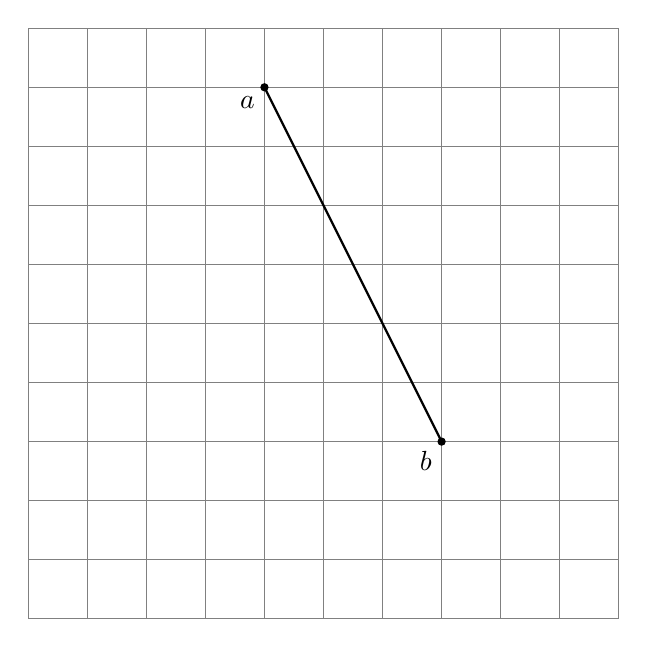
\begin{tikzpicture}[scale=0.75]
    % coordinate system 
    \tkzInit[xmax=5,ymax=5,xmin=-5,ymin=-5]
    \tkzGrid
    \tkzAxeXY
    % coordinates 
    \coordinate [label={below left:$a$}]   (A) at (-1, 4);
    \fill (A)  circle[radius=2pt];
    \coordinate [label={below left:$b$}]   (B) at (2, -2);
    \fill (B)  circle[radius=2pt];
    % lines
    \draw[thick] (A) -- (B); 
\end{tikzpicture}
\end{figure}

% quadrants
% First (x > 0 and y > 0)
% Second (x < 0 and y > 0)
% Third (x < 0 and y < 0)
% Fourth (x > 0 and y < 0)



\section{Monomials and binominals}
A \index{monomial}, also called \index{power product}, is a product of
powers of variables with nonnegative integer exponents. Examples include
\[
-5, 3, 21x, -2x^2, 3a^2b^3
\]
here $-5$ and $3$ are monomial of $x^0$ for any variable $x$

% factor binominals (7x - 1, 9x + 18, ....)

% Quadratics


\subsection{Factoring and multiplying binominals}
When we multiply two binomials such as $(x+4)$ and $(x+2)$ 



With factoring one usually starts with an expression such as
$x^2 + 6 x + 8$ and seeks to transform it into a product of two 
binominals of the form $(x + a)(x + b)$. The original expression is said 
to be of second degree because it contains $x^2$ but no higher power of 
$x$. The factors are first-degree expressions because each contains $x$ but 
no
higher power of $x$. The problem is to find the correct values of $a$ and
$b$ so that the product $(x + a)(x + b)$ will equal the original
expression. We know that
\begin{equation}\label{alg:binom_factor}
x^2 + (a + b)x + ab = (x + a)(x + b)
\end{equation}
Hence to factor the second-degree expression, we should look for two
numbers $a$ and $b$ whose sum is the coefficient of $x$ and whose product
is the constant. Thus to factor $x^2 + 6 x + 8$, we look for two numbers
whose sum is $6$ and whose product is $8$. By mere trial of the possible
factors of $8$ we see that $a = 4$ and $b = 2$ will meet the requirement;
that is: $x^2 + 6 x + 8 = (x + 4)(x + 2)$.

% (h \cdot x + a)(g \cdot x + b) = (h \cdot x)(g \cdot x) + (h \cdot x)b + a(g \cdot x) + (a \cdot b)
% (−3x+1)^2 = x^2 + (-3 + 1)x + (-3 * 1) = x^2 - 2x - 3

\subsection{Quadratic equations}

\section{Polynomials}

\subsection{Polynominal multiplication}

\subsection{Polynominal division}


% Solvr for x and y using elimination. x + 3y = 22, -x + 2y = 8
%If a+b=2 and x+y+z=−4, what is −10x−10y−10b−10a−10z?
%If 6a+3b=−2 and x+8y+z=−9, what is 9z+72y+60a+9x+30b?
\section{Exercises}\label{alg:exercises}
\begin{ExerciseList}

\Exercise Use the distributive property to expand these expressions
\Question $-(6 - \frac{z}{4})$
\Question $-(\frac{1}{2}r + 4)$
\Question $-5(3n + \frac{1}{2})$
\Answer Noting that $-(x + y) = -1 \cdot (x+y) = -x - y$ we see
\begin{enumerate}
\item \myindent $-(6 - \frac{z}{4})   = -6 + \frac{z}{4}$
\item \myindent $-(\frac{1}{2}r + 4)  = -\frac{1}{2}r - 4$
\item \myindent $-5(3n + \frac{1}{2}) = -15n - \frac{5}{2}$
\end{enumerate}

\Exercise Use the distributive property to collect these expressions so
no fractions are within the parentheses
\Question $\frac{3}{5}z - \frac{6}{5}$
\Question $\frac{3}{2} + \frac{7}{8}c$
\Answer We get
\begin{enumerate}
\item \myindent $\frac{3}{5}z - \frac{6}{5} = \frac{3}{5}(z + 2)$
\item \myindent $\frac{3}{2} + \frac{7}{8}c = \frac{1}{8}(12 + 7c)$
\end{enumerate}

\Exercise Determine if the following expressions are equivalent
\Question $9x+6 = 3x+2$
\Question $\frac{5}{2}x - 3 = x+5$
\Question $\frac{\frac{2}{b} + \frac{2}{a}}{\frac{2}{ab}} = a+b$
\Question $\frac{\frac{a}{b} + 1}{\frac{b}{a} - 1} = \frac{a(a+b)}{b(b-a)}$
\Answer We determine equivalent expressions by subtracting them from each
other in order to see if the result becomes zero
\begin{enumerate}
\item \myindent Not equal: $9x + 6 - (3x+2) = 6x - 4$
\item \myindent Not equal: $\frac{5}{2}x - 3 - (x + 5) = \frac{3/2}x - 7$
\item \myindent Equal:
\[
\frac{\frac{2}{b} + \frac{2}{a}}{\frac{2}{ab}} - (a + b) =
\left(\frac{2a + 2b}{ab}\right)\left(\frac{ab}{2}\right) - (a + b) = 0
\]
\item \myindent Equal:
\begin{align*}
\frac{\frac{a}{b}+1}{\frac{b}{a}-1} - \frac{a(a+b)}{b(b-a)} =
\frac{\frac{a}{b} + \frac{b}{b}}{\frac{b}{a} - \frac{a}{a}} - \frac{a(a+b)}{b(b-a)} &= \\
\left(\frac{a + b}{b}\right)\left(\frac{a}{b-a}\right) - \frac{a(a+b)}{b(b-a)} = 0
\end{align*}
\end{enumerate}

\Exercise Expand the expression and combine the like terms:
\Question $6+5(−7n+2)$
\Question $−(−15+2a)+4(8a−6)$
\Question $6(−2+10k)+6(5k−3)$
\Question $1/5 - 2z + z + 2/3$
\Question $7n - (4n - 3)$
\Answer The expressions simplifies to
\begin{enumerate}
\item \myindent $6+5(-7n+2) = -35n + 16$
\item \myindent $-(-15+2a)+4(8a-6) = 30a - 9$
\item \myindent $6(-2+10k)+6(5k-3) = 90k - 30$
\item \myindent $1/5 - 2z + z + 2/3 = 13/15 - z$
\item \myindent $7n - (4n - 3) = 3n + 3$
\end{enumerate}

\Exercise Simplify the following rational expressions by removing their
fractions
\Question $\frac{35n^3}{10n^4}$
\Question $\frac{44a^3}{55a^3}$
\Question $\frac{28y^5}{7y^3}$
\Answer Using the exponent rules from \ref{arit:exp} we get
\begin{enumerate}
\item \myindent $\frac{35n^3}{10n^4} = 3.5n^{-1}$
\item \myindent $\frac{44a^3}{55a^3} = \frac{4}{5}$
\item \myindent $\frac{28y^5}{7y^3} = 4y^3$
\end{enumerate}

\Exercise Write and solve equations to represent the following statements
\Question One half of the quantity represented by $6$ less than a number
$n$ is equal to $17$. Write an equation to represent this statement and
find the value of $n$.
\Question The sum of $3$ consecutive odd numbers is $69$. What is the
first number in this sequence?
\Question $130\%$ of the sum of $7$ and a number $n$ is equal to $91$.
Write an equation to represent this statement and find the value of the
number.
\Question The radiator of a car contains $10$ gallons of liquid $20$
percent of which is alcohol. We want to draw off liquid and replace it
with alcohol so the resulting mixture contains $50$ percent alcohol. How
many gallons of liquid should he draw off?
\Answer We formulate the expressions in terms of their unknown and solve
for it.
\begin{enumerate}
\item \myindent The equation is $17=\frac{n-6}{2}$ and $n = 2 \cdot 17 + 6 = 40$.
\item \myindent We have $n + (n+2) + (n+4) = 69$ and $n = \frac{63}{3} = 21$.
\item \myindent The equation is $\frac{13}{10}(7 + n) = 91$ and $n = 63$
\item \myindent Let $x$ be the amount to be drawn off. Then $10 - x$ is the
gallons remaining of which $\frac{1}{5}$ is alcohol that is $1/5(10 - x)$
is alcohol. After the $x$ gallons are replaced with alcohol, the amount
of alcohol in the tank will be $\frac{1}{5}(10 - x) + x$. As we want this
to be $5$ gallons ($50$ percent alcohol of $10$ gallons) we end up with
\[
\frac{1}{5}(10 - x) + x = 5
\]
Which reduces to
\[
3 \cdot \frac{5}{4} = \frac{15}{4} = \frac{12}{4} + \frac{3}{4} = 3\frac{3}{4}
\]
\end{enumerate}

\Exercise Solve the following linear equations
\Question $\frac{12}{x-12} = \frac{6}{5}$
\Question $\frac{3}{5} = \frac{18}{a + 11}$
\Question $\frac{5}{6} = \frac{k-7}{18}$
\Question $\frac{3}{8} = \frac{15}{t-1}$
\Question $\frac{y-8}{25} = \frac{7}{5}$
\Answer The solutioms are
\begin{enumerate}
\item\myindent $x = \frac{12 \cdot 5}{6} + 12 = 22$.
\item\myindent $a = \frac{18 \cdot 5}{3} - 11 = 19$.
\item\myindent $k = \frac{5 \cdot 18}{6} + 7 = 22$.
\item\myindent $t = \frac{15 \cdot 8}{3} + 1 = 41$.
\item\myindent $y = \frac{7 \cdot 25}{5} + 8 = 43$.
\end{enumerate}

\Exercise Solve these linear inequalities for $x$:
\Question $-12x < 1$
\Question $-18x > -10$
\Question $−16x \geq 13$
\Question $12b - 15 > 21$
\Question $14 - 3x < -1$
\Answer $x$ is
\begin{enumerate}
\item\myindent $x > -\frac{1}{12}$.
\item\myindent $x < \frac{5}{9}$.
\item\myindent $x \leq -\frac{13}{16}$.
\item\myindent $b>3$.
\item\myindent $x>5$.
\end{enumerate}

\Exercise Simplify and solve these linear inequalities for $x$:
\Question $9 - 4d\geq -3$
\Question $9x - 3 < 7x + 4$
\Question $2x + 8 \geq 4x + 5$
\Question $9x + 1 \geq 4x + 2$
\Question $3x + 9 \geq 9x + 10$
\Answer $x$ is
\begin{enumerate}
\item\myindent $d \leq 3$.
\item\myindent $x < \frac{7}{2}$.
\item\myindent $x \leq \frac{3}{2}$.
\item\myindent $x \geq \frac{1}{5}$
\item\myindent $x \leq -\frac{1}{6}$
\end{enumerate}

\Exercise Name the quadrants of these coordinates
\Question $(1,1)$
\Question $(-1,1)$
\Question $(-1,-1)$
\Question $(1,-1)$
\Question $(0,0)$ 
\Answer The quadrants are
\begin{enumerate}
\item\myindent First quadrant
\item\myindent Second quadrant
\item\myindent Third quadrant
\item\myindent Fourth quadrant
\item\myindent The origin has no quadrant.
\end{enumerate}

\Exercise Multiply these binomials
\Question $(x-3)^2$ 
\Question $(x-3)(x+10)$ 
\Question $(x+8)^2$ 
\Question $(x+1)(x-4)$ 
\Question $(x+9)^2$ 
\Answer Using \ref{alg:binom_factor} we get the following quadratics 
\begin{enumerate}
\item\myindent $(x-3)^2 = x^2 + (-3 + -3)x + (-3 \cdot -3) = x^2 - 6x + 9$
\item\myindent $(x-3)(x+10) = x^2 + (-3 + 10)x + (-3 \cdot 10) = x^2 + 7x - 30$
\item\myindent $(x+8)^2 = x^2 + (8+8)x + (8\cdot8) = x^2 + 16x + 64$
\item\myindent $(x+1)(x-4) = x^2 + (1 + -4)x + (1 \cdot -4) = x^2 - 3x - 4$
\item\myindent $(x+9)^2 = x^2 + (9+9)x + (9\cdot9) = x^2 + 18x + 81$
\end{enumerate}

\Exercise Factor the following expressions. 
\Question $x^2 + 9x + 20$
\Question $x^2 + 5x + 6$
\Question $x^2 - 5x + 6$
\Question $x^2 - 9$
\Question $x^2 + 7x - 18$
\Answer Using \ref{alg:binom_factor} we get the following factors 
\begin{enumerate}
\item\myindent $x^2 + 9x + 20 = x^2 + (4 + 5)x + (4\cdot5) = (x+4)(x+5)$.
\item\myindent $x^2 + 5x + 6 = x^2 + (3 + 2)x + (2\cdot3) = (x+2)(x+3)$.
\item\myindent $x^2 - 5x + 6 = x^2 + (-3 + -2)x + (-2\cdot-3) = (x-2)(x-3)$.
\item\myindent $x^2 - 9 = x^2  + (-3 + 3)x + (-3\cdot3) = (x-3)(x+3)$.
\item\myindent $x^2 + 7x - 18 = x^2 + (-2 + 9)x + (-2\cdot9) = (x+9)(x-2)$.
\end{enumerate}

\end{ExerciseList}

\chapter{Elementary number theory}
% TODO number theory missing concepts
% - (essential to proof of correctness of euclids algorithm)

% TODO extended missing concepts
% greatest common denomijator and least common muktiple

% - Newton's generalised binomial theorem
% - Add info about binominal theorem limitations (such as only integers)
% - Use binominal thorem to evaluate fractional powers
% - fundamental theorem of arithmetic: that every natural number greater than 1 is either prime,
% or else can be expressed as a product of primes in a way which is unique except for the order
% in which the primes are arranged.
% - the prime numbers are the basic building blocks from which all the natural numbers are constructed .
%% Fermat's Little Theorem
%% A number is divisible by another number (a divisor) if its prime factorization contains the prime factorization of the divisor. All numbers which divide such a number will have a factorization which is part of
%% Of particular interest in the non-negative integers i.e. elements of the set $\{0,1,2,3...\}}$, also known as the natural numbers and usually abbreviate as $\N$.
%% - phi and e are irrational
%% - prime counting function
%% - eliptic curves
%% - enhanced prime finding and locating algorihms (sqare root of n}
%% - one way functions and cryptography (RSA - the code book)
%% - Mesanine primes: Numbers that can be obtained by raising 2 to a power and then subtracting 1 are called Mersenne numbers, for reasons I’ll give later in the chapter. Prime numbers of this particular form are called Mersenne primes
% [BINOMAL]
%http://www.mcs.sdsmt.edu/ecorwin/finite_structures/bin_thm/bin_thm.html
%http://en.wikipedia.org/wiki/Binomial_theorem#Simple_derivation
%http://planetmath.org/encyclopedia/InductiveProofOfBinomialTheorem.html
%http://www.intmath.com/Series-binomial-theorem/4_Binomial-theorem.php
%http://www.matheclipse.org/en/Binomial_coefficient
%http://en.wikipedia.org/wiki/Binomial_coefficient#Combinatorial_interpretation

% https://en.wikipedia.org/wiki/Lindemann–Weierstrass_theorem#Transcendence_of_e_and_.CF.80 proof that pi and e and sin is not algebraic
% - http://planetmath.org/sites/default/files/texpdf/39438.pdf
% - http://www.math.brown.edu/~res/MathNotes/notes5.pdf
% - http://www.maths.bris.ac.uk/~malab/PDFs/MA469.pdf
% - https://www.math.leidenuniv.nl/scripties/BachWarrens.pdf

% primality tests http://math.stackexchange.com/questions/4597/simple-explanation-and-examples-of-the-miller-rabin-primality-test

% proof that e and pi is irrational then that they are trancedental

% Chinese remainder theorem http://en.m.wikipedia.org/wiki/Chinese_remainder_theorem

% Sieve of Eratosthenes algorithm impelementation

In number theory we deal with the properties of various classes of numbers such as the integers, which is any number that can be written without a fractional or decimal component and is denoted with the the symbol $\mathbb{Z}$. Thus,$-7$, $0$, and $2$ are integers; $1.7$ and $\frac{1}{7}$ are not. Incidentally the Latin word "integer" literally means "untouched", hence "whole". Of particular interests is the set of all positive integers, also known as the natural numbers and symbolised by $\mathbb{N}$.

\section{Basic properties of Integers}
Let us first consider that integers are either $even$ or $odd$, formally we write:
\begin{definition}\label{num_def}
The $even$ numbers are the numbers written on the form $2k$ and the $odd$ numbers are the numbers written on the form $2k+1$ where $k$ is any integer.
\end{definition}
some arithmetic can convince us that this indeed yields the desired numbers:
\[
\begin{array}{lcl}
2 \cdot 0     & = & 0 \\
2 \cdot 0 + 1 & = & 1 \\
2 \cdot 1     & = & 2 \\
2 \cdot 1 + 1 & = & 3 \\
:             &   & :
\end{array}
\]

The $odd$ numbers may also be expressed as being either one more than a
multiple of $4$ or three more than a multiple of $4$. Symbolically, we can say
that they are either of the form $4k + 1$ or of the form $4k  + 3$. Again some
examples clarifies the smoke
\[
\begin{array}{lcl}
4 \cdot 0 + 1 & = & 1 \\
4 \cdot 0 + 3 & = & 3 \\
4 \cdot 1 + 1 & = & 5 \\
4 \cdot 1 + 3 & = & 7 \\
:             &   & :
\end{array}
\]

incidentally this shows that when we divide a $odd$ number by $4$, we must get
a remainder of either $1$ or $3$ \label{remainder}. Armed with this knowledge
we can shine some light on the properties of $odd$ numbers:
\begin{corollary}
The square of an $odd$ number is $odd$
\end{corollary}
\begin{proof}
Consider, by \ref{num_def}, the algebraic form of the square of an odd number
\[
\begin{array}{lcl}
(2k+1)^2 & = & (2k)^2 + 2(2k) + 1 \\
                 & = & 4(k^2 + k) + 1
\end{array}
\]
The last expression being on the form $4k + 1$ yields the desired result.
\end{proof}

Integers can be used to construct another class of numbers, known as the rational numbers. Here we say a 'rational number' is a fraction $\frac{a}{b}$, where $a$ and $b$ are integers; we may suppose that $a$ and $b$ have no common factor (since if the had we could remove it) and that $b$ does not equal zero. We denote these numbers by $\mathbb{Q}$ for quotient. With only these properties at hand we can move on to prove one of mathematics first great results; that $\sqrt{2}$ is irrational.
\begin{proposition}
$\sqrt{2}$ is irrational.
\end{proposition}
\begin{proof}
To say that $\sqrt{2}$ is irrational is the same as saying $2$ cannot be expressed in the form $\left(\frac{a}{b}\right)^2$ or that the equation
\begin{equation}\label{2_irrational}
a^2 = 2b^2
\end{equation}
cannot be satisfied by integral values of $a$ and $b$ without any common factor. Let us for sake of eventual contradiction suppose that \ref{2_irrational} is true for some $a$ and $b$, then it follows that $a^2$ is even (since $2b^2$ is divisible by $2$) and thus that $a$ is even (since the square of an even number is even). If $a$ is even then
\[
a = 2c
\]
for some integral value of $c$; and therefore
\[
 a^2 = 2b^2 = (2c)^2 = 4c^2
\]
or
\[
b^2 = 2c^2
\]
Hence $b^2$ is also even and therefor $b$ is even. Now since both $a$ and $b$ are even they must have the common factor $2$. This contradicts our hypothesis, and therefore the hypothesis is false
\end{proof}
Notice how this proof is by \emph{reductio ad absurdum}, a proof style much beloved by the greeks and one of mathematics finest weapons. In these types of proofs we attack our theorem by taking an assumption and then show that it leads to a contradiction and hence is false.

\myindent Now since we have proved that $\sqrt{2}$ cannot be written as a fraction can we then find another way to express it ?. By definition, a number is $algebraic$ (denoted by $\mathbb{A}$) if it is the solution to some polynomial equation
\[
a_{n}x^{n} + a_{n-1}x^{n-1} + \cdots + a_{2}x^{2} + a_{1}x + a_0 = 0
\]
where all the coefficients $a_n, a_{n-1}, \cdots, a_2, a_1$ and $a_0$ are integers. Now as $\sqrt{2}$ is the solution to the polynomial $x^2 - 2 = 0$ it follows that it is a irrational algebraic number. Also as any integer $k$ is a solution to $x-k=0$ we see that all integers are algebraic and hence $\mathbb{Z} \in \mathbb{A}$. Later we shall meet another class of numbers known as transcendental numbers $\mathbb{T}$ which is simply the set of all non-algebraic numbers. As it turns  out almost all irrational numbers are transcendental and all transcendental numbers are irrational. The box below should hopefully clarify the relationships between these various sets of numbers
\begin{figure}[htb!]
\begin{center}
% TODO draw with tikz
%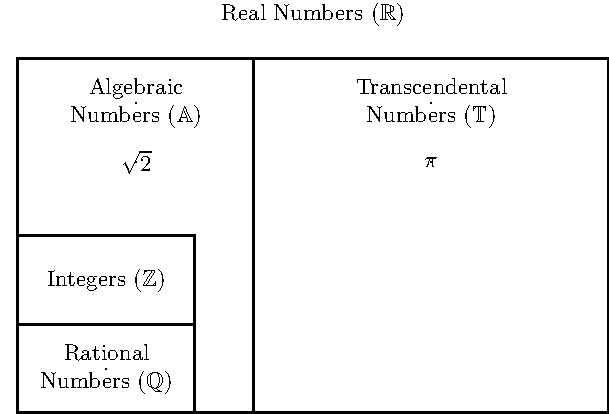
\includegraphics[width=10cm]{images/number_types.pdf}
\end{center}
\end{figure}
Note how all of these numbers are contained in the set of real numbers $\mathbb{R}$. The real numbers thus includes both integers and rational numbers, such as $42$ and $\frac{1}{3}$, and transcendental numbers, such as $\pi$ and irrational algebraic numbers such as $\sqrt{2}$. Informally we may think of real numbers as any number with or without a decimal point that may contain an infinite decimal tail that continue in some way.

\section{Divisibility}
The integer $n$ is divisible by $m$ if the ratio $n/m$ is an integer. Hence we write $m|n$ when $m$ divides $n$ evenly and define
\begin{equation}\label{divisibility}
m|n \Longleftrightarrow m > 0 \textnormal{ and } n = mk
\textnormal{ for some integer } k
\end{equation}

How do we know if a number is divisible by some other number ?. Here we are out of luck, in general we can only answer this by doing full division and checking if the remainder is zero. Mathematics contains many functions that are easy to do (such as multiplication and differentiation) but hard to undo (such as division and integration). Later on we will see that exactly this property of division can be used to craft a simple scheme for secure communication. For now let us extract some useful properties from the above definition of divisibility.
\begin{proposition}
If $a > b$ and $n$ divides $a$ and $b$ evenly then it also divide their
difference.
\end{proposition}
\begin{proof}
By \ref{divisibility} we have $a = nx$ and  $b = ny$ for some integral value of $x$ and $y$. Thus $a-b = nx - ny = n(x-y)$ as desired.
\end{proof}

As remarked on page \pageref{remainder} not all numbers divides evenly:
\begin{proposition}\label{division_algorithm}
If $a$ and $b$ are integers with $b\neq0$, then there is a unique pair of integers $q$ and $r$ such that
\[
a = qb+r \textnormal{ and } 0 \leq r \leq |b|
\]
\end{proposition}
Note that
\[
\frac{a}{b} = q + \frac{r}{b}
\]
where for $b>0$ we have $0 \leq \frac{r}{b} < 1$ and for $b<0$ we have $0 \geq \frac{r}{b} > -1$. As example the division $9/4$ with $a=9$ and $b=4$ becomes $9=2\cdot4 + 1$ giving us the quotient $q=2$ and remainder $r=1$
\begin{proof}
Our job is to prove that the numbers $q$ and $r$ exists, known as existence and that they are unique, also known as uniqueness. First we prove existence. Let
\[
S = \{a-nb|n \in \mathbb{Z}\} = {a,a \pm b,a \pm 2b,...}
\]
\end{proof}

\section{Euclid's Algorithm}
% GCD
The greatest common divisor of integers a and b, denoted by gcd(a,b), is the largest integer that divides (without remainder) both a and b. So, for example:

gcd(15, 5) = 5,	gcd(7, 9) = 1,	gcd(12, 9) = 3,	gcd(81, 57) = 3.

It is well known that if the gcd(a, b) = r then there exist integers p and s so that:

p(a) + s(b) = r.
By reversing the steps in the Euclidean Algorithm, it is possible to find these integers p and s. We shall do this with the above example:
Starting with the next to last line, we have:

3 = 9 -1(6)
From the line before that, we see that 6 = 24 - 2(9), so:
3 = 9 - 1(24 - 2(9)) = 3(9) - 1(24).
From the line before that, we have 9 = 57 - 2(24), so:
3 = 3( 57 - 2(24)) - 1(24) = 3(57) - 7(24).
And, from the line before that 24 = 81 - 1(57), giving us:
3 = 3(57) - 7( 81 - 1(57)) = 10(57) -7(81).
So we have found p = -7 and s = 10.

The procedure we have followed above is a bit messy because of all the back substitutions we have to make. It is possible to reduce the amount of computation involved in finding p and s by doing some auxillary computations as we go forward in the Euclidean algorithm (and no back substitutions will be necessary). This is known as the extended Euclidean Algorithm.

%http://www.math.utah.edu/~fguevara/ACCESS2013/Euclid.pdf
%http://pages.pacificcoast.net/~cazelais/222/xeuclid.pdf
Euclid devised a clever algorithm for locating the greatest common divisor.
% TODO GCD and LCM
% TODO add proof
\begin{algorithm}
    \caption{Euclid’s algorithm}
    \label{euclid}
    \begin{algorithmic}[1] % tells where the line numbering should start
        \Procedure{Euclid}{$a,b$} \Comment{The g.c.d. of a and b}
            \State $r\gets a \bmod b$
            \While{$r\not=0$} \Comment{We have the answer if r is 0}
                \State $a \gets b$
                \State $b \gets r$
                \State $r \gets a \bmod b$
            \EndWhile\label{euclidendwhile}
            \State \textbf{return} $b$\Comment{The gcd is b}
        \EndProcedure
    \end{algorithmic}
\end{algorithm}

\section{Primes}
A prime number is a natural number greater than 1 that cannot be formed by multiplying two smaller natural numbers. A natural number greater than 1 that is not prime is called a composite number. For example, $5$ is prime because the only ways of writing it as a product, $1 \cdot 5$ or $5 \cdot 1$. On the other hand $10$ is a composite as it can be written as $2 \cdot 5$. Semilarly 666 is not a prime as 
\[
666 = 2 \cdot 3 \cdot 3 \cdot 37
\]
 The first primes are
\[
2, 3, 5, 7, 11, 13, 17, 19, 23, 29, 31, 37 ...
\]
As we shall se later there are infintly many prime numbers. Prime numbers are thus important as they serve as the building blocks of other integers, indeed the following holds true:

\begin{proposition}\label{prim_div}
Every integer n $>$ 1 is divisible by at least one prime
\end{proposition}
\begin{proof}
Let $A$ be a composite number (i.e. non prime). By definition there must be some smaller number $B$ dividing evenly into $A$, where 1 $<$ $B < A$. Now either $B$ is prime or it is not. If $B$ is prime, then the original number $A$ indeed has a prime divisor, as claimed. Otherwise, $B$ is not prime and so has a divisor, say $C$, with $1 < C < B <$ A. If $C$ is prime, we are done, for $C$ divides evenly into $B$, and $B$ divides evenly into $A$. If $C$ is composite then it must have a proper divisor, $D$, and thus we continuously arrive at:
\[
A > B > C > D > ... > 1
\]
But all of these are positive integers, so we must reach a point in which we find a prime. Therefor any number, which is not prime itself, is divisible by at least one prime (usually, of cause, by several).
\end{proof}

If one surveys the list of the first 50 primes
\begin{lstlisting}
2, 3, 5, 7, 11, 13, 17, 19, 23, 29, 31, 37,
41, 43, 47, 53, 59, 61, 67, 71, 73, 79, 83,
89, 97, 101, 103, 107, 109, 113, 127, 131,
137, 139, 149, 151, 157, 163, 167, 173, 179,
181, 191, 193, 197, 199, 211, 223, 227, 229
\end{lstlisting}
then apparently the primes seams to be getting scarcer as the numbers go larger. Indeed between the numbers $1$ and $1000$ there are $168$ primes, whereas between $9000$ and $10.000$ there is but $112$. At first this seams logical enough since small numbers only have few possible factors and thus higher likelihood of being primes, yet one cannot help ask if we will ever reach such large numbers that the primes may eventually run out completely, rendering all subsequent numbers composite. Luckily this question had already been answered by the great greek mathematician Euclid who 300 B.C. in his IX book as proposition 20 indeed claimed:

\begin{proposition}
Prime numbers are more than any assigned multitude of prime numbers.
\end{proposition}
Euclid's terminology sounds strange, but what he is really proposing is that the sequence of primes does not end.
\begin{proof}
Let us for sake of eventual contradiction suppose that there is only a finite number of primes and that
\[
2, 3, 5, ..., P
\]
is the complete series (so that $P$ is the largest prime); and let us, on this hypothesis, consider the number $Q$ defined by the formula
\[
Q = (2 \cdot 3 \cdot 5 \cdots P) + 1
\]
It is plain that $Q$ is not divisible by any of $2, 3, 5, ..., P$; for it leaves the remainder $1$ when divided by any one of these numbers. But, if $Q$ is not prime, then by \ref{prim_div} it is divisible by some prime, and therefore there is a prime (which may be $Q$ itself) greater than any of them. This contradicts our hypothesis, that there is no prime greater than $P$; and therefore this hypothesis is false.
\end{proof}

Finding and counting primes is a long standing hobby for mathematicians, and one might ask if it can be automated. One such method was discovered by the greek mathematician Eratosthenes (ca. 284-192 B.C.) who as the chief librarian at the great Library at Alexandria spend much of his time studying mathematics, astronomy and philosophy. His method (known as Eratosthenes sieve) is as follows; write a list of all the consecutive integers, starting with $2$, among which you want to find the primes. As $2$ is prime, cross all subsequent multiples off. The next integer that has not yet been crossed of (3) must then also be prime and so we can eliminate all of its multiples. As we continue in this manner we will clearly sieve out all composite numbers and be left with the primes.
\begin{verse}\emph{
Sift the Twos and sift the Threes,\\
The Sieve of Eratosthenes.\\
When the multiples sublime,\\
The numbers that remain are Prime.}
\end{verse}
although this method will indeed generate the primes, it is not as efficient as one might have liked (although optimized and more complex methods exists). Later we shall encounter the prime counting function $\pi(n)$, which outputs the number of primes less than or equal to a given number $n$ (the use of $\pi$ in this function is an unfortunate standard as it has nothing to do with the well known geometric constant $3.1415...$).


\section{Modulo arithmetic}
% TODO missing modulo arithmetic
% - definition and excercises from http://www.math.rutgers.edu/~erowland/modulararithmetic.html
% - explain (perhaps in excercises) why the divisibility tests works
% - excercises
% --- sum of two even numbers is even
% --- the sum of an even and odd number is odd
% --- the product of two even numbers are even
As mentioned before integers can be broken up into the classes of even $..–6, –4, –2, 0, 2, 4, 6..$ and odd numbers $..–5, –3, –1, 1, 3, 5..$ There are certain generalisations we can make about the arithmetic of numbers based on which of these two classes they come from. For example, we know that the sum of two even numbers is even. The sum of an even number and an odd number is odd. The sum of two odd numbers is even. The product of two even numbers is even, etc.

Now we represent each of our two classes by a single symbol. We let the symbol "$0$" mean "the class of all even numbers" and the symbol "$1$" mean "the class of all odd numbers". The statement "the sum of two even numbers is even" can then be expressed by the following:
\[
0 + 0 \equiv 0 \textrm{ mod } 2.
\]
Here, the "$\equiv$" symbol is not equality but congruence, and the "$\textrm{mod} 2$" just signifies that our modulus is $2$. The above statement is read "Zero plus zero is congruent to zero, modulo two." The statement "the sum of an even number and an odd number is odd" is represented by
\[
0 + 1 \equiv 1 \textrm{ mod } 2.
\]
Those examples are natural enough. But when we try to express the statement "the sum of two odd numbers is even"? we get this strange looking expression
\[
1 + 1 \equiv 0 \textrm{ mod } 2.
\]
We have analogous statements for multiplication:
\begin{align*}
0 \cdot 0 &\equiv 0 \textrm{ mod } 2 \\
0 \cdot 1 &\equiv 0 \textrm{ mod } 2 \\
1 \cdot 1 &\equiv 1 \textrm{ mod } 2
\end{align*}
Basically we now have a number system with addition and multiplication but in which the only numbers that exist are 0 and 1. You may ask what use this has. Well, our number system is the system of integers modulo 2, and because of the previous six properties, any arithmetic done in the integers translates to arithmetic done in the integers modulo 2.

Since any integer solution of an equation reduces to a solution modulo 2, it follows that if there is no solution modulo 2, then there is no solution in integers. For example, assume that a is an integer solution to
\[
2a – 3 = 12,
\]
which reduces to
\[
0 \cdot a + 1 \equiv 0 \textrm{ mod } 2,
\]
or $1 \equiv 0 \textrm{ mod } 2$. This is a contradiction since no even number is an odd number. Therefore the above congruence has no solution, so a couldn't have been an integer. This proves that the equation $2a – 3 = 12$ has no integer solution.

\section{Exercises}
\begin{ExerciseList}

\Exercise What is the lowest number divisible by both $12$ and $20$
\Answer Numbers divisible by $12$ and $20$ also have to be divisible by each of their prime factors $12 = 2 \cdot 2 \cdot 3$ and $20 = 2 \cdot 2 \cdot 5$ thus $2 \cdot 2 \cdot 3 \cdot 5 = 60$.

\Exercise In 2000 the Jordanian mathematician, Murad A. AlDamen devised the following method for testing divisibility \pagenote{Found on the prime puzzlers project, at: \url{http://www.primepuzzles.net/puzzles/puzz_101.htm}}
\Question Use Murad's method to determine if $61$ divides $3598207$
\Question Prove Murad's method.
\Answer TODO
\end{ExerciseList}

\printpagenotes*


%Let L*M=N =n1+10n2, L(k1+10k2)=n1+10n2
%L*k1-n1=10a É.(1)
%-10Lk2=10a-10n2, Lk2=a-n2
%n2 ÐLk2=a É (2)
%add one to two and by N=M*L
%we find ((n1+10n2)(k1-k2)+ (k1+10k2)(nn-n1))/(k1+10k2)=11a, then (n2k1-k2n1)=0 (mod M)

% Divisibility rules excercieses
% http://mathforum.org/kb/message.jspa?messageID=1461184

% Binominal theorem excercises
% http://www.purplemath.com/modules/binomial2.htm

% GCF excercises
% Each time Miranda goes to the store she plans to spend $7, and each time Savannah goes to the store she plans to spend $9. A few weeks from now, Miranda and Savannah are surprised to find out that they have spent the exact same total amount of money at the store.

\chapter{Combinatorics}\label{combi}
% TODO missing combinatorics
% - explain why For example, the number of ways to deal a hand of five cards from a deck of 52 is C(52, 5) = 52! / 5! 47! = 2,598,960.
% - Ramsey theory http://en.m.wikipedia.org/wiki/Ramsey_theory
% - Ramsey theorem http://en.m.wikipedia.org/wiki/Ramsey%27s_theorem
% - Van der Waerden's theorem http://en.m.wikipedia.org/wiki/Van_der_Waerden%27s_theorem
% - https://medium.com/@arankhanna/the-proof-of-wagner-s-conjecture-and-why-it-matters-ff5c7c9b9425
% design theory
% - http://www.wired.com/2015/06/answer-150-year-old-math-conundrum-brings-mystery/
% fano plane (perhaps move to geometry)

% TODO A tree diagram consists of branches corresponding to the outcomes of two or more probability experiments that are done in sequence.
% A coin is tossed and a die is rolled. Draw a tree diagram and find the total number of outcomes. They are H1, H2, H3, H4, H5, H6, T1, T2, T3, T4, T5, T6.
% TODO draw two tree diagrams
% Three coins are tossed. Draw a tree diagram and find the sample space. the sample space is HHH, HHT, HTH, HTT, THH, THT, TTH, TTT.
% TODO table based methods, for example table of outcomes for two dies or deck of card (introduce ordeered pair)

% http://reference.wolfram.com/language/Combinatorica/ref/DeBruijnSequence.html
% The sequence can be used to shorten a brute-force attack on a PIN-like code lock that does not have an "enter" key and accepts the last n digits entered. For example, a digital door lock with a 4-digit code would have B(10, 4) solutions, with length 10000. Therefore, only at most 10000 + 3 = 10003 (as the solutions are cyclic) presses are needed to open the lock. Trying all codes separately would require 4 × 10000 = 40000 presses.



Combinatorics is one of the most fascinating and frustrating branches of mathematics. Many excellent students find it impossibly difficult while some find it as easy as breathing. Classically, combinatorics deals with finite sets of objects and the various ways their subsets and their elements can be counted and ordered.

One of the first formal attempts of combinatorial thinking seems to have come around $960$, when \index{Bishop Wibold of Cambrai} correctly enumerated the $56$ outcomes that can arise when three dice are thrown simultaneously: $\{1, 1, 1; 1, 1, 2; 1, 1, 3, ...\}$ and so on. A thirteenth-century Latin poem, \index{DeVetula}, listed the $216 (= 6 \cdot 6 \cdot 6)$ outcomes that may result when three dice are thrown in succession.

If the results $56$ and $216$ seams somewhat unclear, don't despair this chapter will teach you how to arrive at these results safely on your own.

 % TODO explain why the first is 56 and the second 216

So, in Mathematics we use more precise language:

	If the order doesn't matter, it is a Combination.
	If the order does matter it is a Permutation.

A Permutation is an ordered Combination.

\section{Permutations}
In other words:

You've decided to take $3$ steps and randomly choose left or right as the direction each time. How many different outcomes exists?. The mathematical branch of combinatorics helps us answers questions such as these and its mastery is essential to study statistics. Returning to our example we notice that you have two possibilities for the first step, two possibilities for the second and again two possibilities for the third yielding $2 \cdot 2 \cdot 2 = 8$ possible outcomes. The figure below shows the situation:
\begin{figure}[H]
\centering
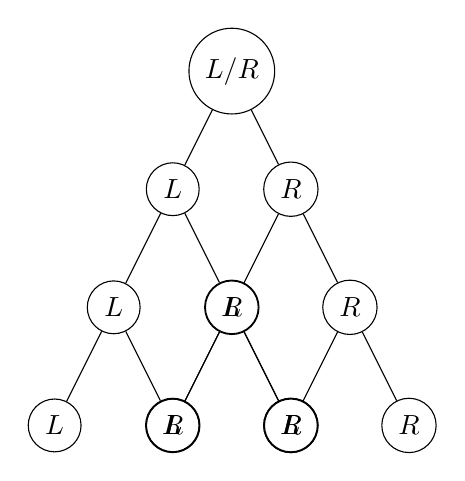
\begin{tikzpicture}
\node[circle,draw](1){$L/R$}
  child {
      node [circle,draw](2){$L$}
         child {
             node [circle,draw](3){$L$}
                   child { node [circle,draw](4){$L$}}
                   child { node [circle,draw](5){$R$}}
         }
         child {
             node [circle,draw](6){$R$}
                   child { node [circle,draw](7){$L$}}
                   child { node [circle,draw](8){$R$}}
         }
   }
   child {
       node [circle,draw](9){$R$}
         child {
             node [circle,draw](10){$L$}
                   child { node [circle,draw](11){$L$}}
                   child { node [circle,draw](12){$R$}}
         }
         child {
             node [circle,draw](13){$R$}
                   child { node [circle,draw](14){$L$}}
                   child { node [circle,draw](15){$R$}}
         }
   };
\end{tikzpicture}
\end{figure}

Suppose we have before us 2 red aces and 2 red kings from the usual deck of 52 cards. How many different pairs consisting of one ace and one king can be put together? Since each ace can be paired with either of 2 kings, there are 2 different pairs for any one ace. Since we have 2 aces, there are $2 \cdot 2$ or 4 different pairs.

\section{Counting selections}
Consider in how many ways can we arrange the set $\{1,2,3\}$:
\[
\{1, 2, 3\}, \{1, 3, 2\}, \{2, 1, 3\}, \{2, 3, 1\}, \{3, 1, 2\}, \{3, 2, 1\}
\]
that is we have $3$ ways of choosing the first element, and $3-1$ options for the second (as we cannot repeat the first choise) and $3-2$ for the last (as non of the former two choices may be used), therefor we can arrange them in $3 \cdot 2 \cdot 1 = 6$ ways. In general we define the number of permutations of a set with $n$ elements as the faculty function $n!$
\[
n! = n \cdot (n-1) \cdot (n-2) \cdots  (n - (n -1)) = 1 \cdot 2 \cdots n = \prod_{k=1}^{n}k,
\]

the last notation simply means that we multiply all the values of $k$ from $1$ to $n$. A recursive version (a self-calling function) can be constructed by noting that $n! = n(n-1)!$. \\

\myindent Now consider a slightly more complex question: in how many ways can we pick two elements from the set $\{1,2,3\}$, the answer turns out to be three ways:
\[
\{1, 2\}, \{1, 3\}, \{2, 3\}
\]
To generalize this we can ask in how many ways can we pick a unordered subset with $k$ elements from a set with $n$ elements ?. To answer this, observe there are $n$ choices for the first element and for each of these there are $n - 1$ choices for the second; and so on until there are $n - k + 1$ for the k'th element. That is we have $n \cdot (n-1) \cdots (n - k + 1)$ ways for picking a $k$-element subset from $n$. As we are picking unordered sets and since each $k$-element subset has exactly $k!$ different orderings, we get our answer by dividing with $k!$:
\begin{equation}\label{binom}
\binom{n}{k} = \frac{n(n-1) \cdots (n - k + 1)}{k!},  \qquad \text{integer } n \geq k \geq 0
\end{equation}
and if we multiply the numerator and denominator of \ref{binom} by $(n - k)!$ we get:
\[
\frac{n(n-1) \cdots (n - k + 1)}{k!} \cdot \frac{(n - k)!}{(n - k)!} =  \frac{n!}{k!(n-k)!}
\]
The symbol $\binom{n}{k}$ is known as a binomial coefficient and we read it "$n$ choose $k$" (the number of ways to select $k$ elements from $n$ element set). Using this result we can directly answer the above question of how many ways to choose two elements from a three element set:
\[
\binom{3}{2}  = \frac{3!}{2! (3-2)!} = \frac{3 \cdot 2 \cdot 1}{2 \cdot 1 \cdot 1} = 3
\]
Interestingly when determining the number of ways to pick $k$ elements we have in effect also specified the $n-k$ unchosen things, therefore
\begin{equation}\label{binom_symmetry}
\binom{n}{k} = \binom{n}{n-k}
\end{equation}
this symmetry can be observed in the above example where we have $3$ ways of picking $2$ elements from a $3$-element set but then also $3$ ways of picking the remaining element. It also follows directly from the definition of the binomial coefficient
\[
\binom{n}{k} =  \frac{n!}{k!(n-k)!} =  \frac{n!}{(n-(n-k))!(n-k)!} = \binom{n}{n-k}
\]

\myindent Another rather remarkable result, known as Pascal's rule, can be derived by marking a particular object $\epsilon$ in an $n$-element set. Now if we pick $k$ objects from $n$, then either $\epsilon$ is picked or it is not. If $\epsilon$ is in the subset then there is $k-1$ objects left to choose among the $n-1$ elements, or more formally $\binom{n-1}{k-1}$. If $\epsilon$ is not in the subset, we need to choose all the $k$ elements in the subset from the $n-1$ objects that are not $\epsilon$; formally that is $\binom{n-1}{k}$. Thus there are
\[
\binom{n-1}{k-1} + \binom{n-1}{k}
\]
ways to choose $k$ elements from $n$ depending on whether $\epsilon$ is included in each selection or not. But this number must be the same as the binomial coefficient and thus we get:
\begin{equation}\label{pascal_rule}
\binom{n}{k}  = \binom{n-1}{k-1} + \binom{n-1}{k}
\end{equation}
this result can also be arrived at by algebraic manipulation
\begin{align*}
 \binom{n-1}{k-1} + \binom{n-1}{k}
& =  \frac{(n-1)!}{(k-1)!((n-1)-(k-1))!} + \frac{(n-1)!}{k!((n - 1) - k)!} \\
& =  \frac{(n-1)!}{(k-1)!(n-k)!} + \frac{(n-1)!}{k!(n - (k + 1))!} \\
& =  \frac{k(n-1)!}{k!(n-k)!} + \frac{(n-1)!(n-k)}{k!(n - k)!} \\
& =  \frac{(n-1)!(k + n - k)}{k!(n-k)!} \\
& =  \frac{n!}{k!(n-k)!}
\end{align*}

%% PASCALs TRIANGLE
\myindent From Pascal's rule we can construct his famous triangle. Observe that according to this rule (see \ref{pascal_rule}) you can calculate $\binom{5}{3}$ as:
\begin{align*}
 \binom{5}{3}
& =  \binom{4}{3} + \binom{4}{2}  \\
& =  \binom{4}{3} + \binom{3}{2} +  \binom{3}{1} \\
& =  \binom{4}{3} + \binom{3}{2} +  \binom{2}{1} + \binom{2}{0} \\
\end{align*}
as $\binom{2}{0} = 1$, we can stop the expansion. In general as $\binom{n}{n}$ and $\binom{n}{0}$ are always $1$ (when $n \geq 0$) we are guarantied that the expansion always terminates. Thus we have found a convenient way of expressing higher binomial coefficients as sums of consecutive smaller ones:
\begin{center}
\begin{tabular}{l|*{5}{c}r}
\toprule
$n$ & $\binom{n}{0}$        & $\binom{n}{1}$ & $\binom{n}{2}$ & $\binom{n}{3}$ & $\binom{n}{4}$  & $\binom{n}{5}$ \\
\hline
0		& 1                     & 0 			       & 0 			        & 0 			       & 0 			         & 0   \\
1   & 1                     & 1 			       & 0 			        & 0 			       & 0  			       & 0   \\
2   & 1                     & 2 			       & 1 			        & 0 			       & 0  			       & 0   \\
3		& 1                     & 3 			       & 3 			        & 1			         & 0  			       & 0   \\
4		& 1                     & 4 			       & 6 			        & 4			         & 1  			       & 0   \\
5		& 1                     & 5 			       & 10 			      & 10			       & 5  			       & 1   \\
\bottomrule
\end{tabular}
\end{center}
discarding the zero's we can arrange these numbers into a triangle:
\[
\begin{array}{c}
1 \\
1\ \myindent 1\\
1\ \myindent 2\ \myindent 1   \\
1\ \myindent 3\ \myindent 3\   \myindent 1   \\
1\ \myindent 4\ \myindent 6\   \myindent 4\   \myindent 1\\
1\ \myindent 5\ \myindent 10\ \myindent 10\ \myindent 5\ \myindent1\\
\ \textnormal{and so on} \ \\
\end{array}
\]
where the next row must contain:
\[
\binom{6}{0} \myindent \binom{6}{1} \myindent \binom{6}{2} \myindent \binom{6}{3} \myindent \binom{6}{4} \myindent \binom{6}{5} \myindent \binom{6}{6}
\]
but we already know that expressions like $\binom{6}{1}$ can be rewritten to
$\binom{5}{1} + \binom{5}{0} = 5 + 1$. So we see that each entry in the new row
is obtained simply by adding the numbers in the row above to the left and right.
\[
1\ \myindent 6\ \myindent 15\ \myindent 20\ \myindent 15\ \myindent 6\ \myindent 1
\]

To generate the triangle, you start with a 1, and then immediately below it, you put two 1’s, one to either side. Then for each successive row, you put a new 1 at either end and complete the row between them by adding together each adjacent pair of entries in the row above and putting their sum halfway between them.

% TODO binomials (a+b)^2 = 1 2 1, (a+b)^3 = 1 3 3 1

\newpage
%%
\section{Newton's Binomial Theorem}
In mathematics a binomial is a polynomial with two terms, i.e such as these
\[\begin{array}{lcl}
(a + b)^0 &=& 1\\
(a + b)^1 &=& a + b \\
(a + b)^2 &=& a^2 + 2ab + b^2 \\
(a + b)^3 &=& a^3 + 3a^2b + 3ab^2 + b^3 \\
(a + b)^4 &=& a^4 + 4a^3b + 6a^2b^2 + 4ab^3 + b^4 \\
:                &   & :
\end{array}\]
or in general
\[
(a+b)^n = \overbrace{(a+b)(a+b)\cdots(a+b)}^{n\textnormal{ factors}}
\]
the relationship between such polynomials and combinatorics stems from the so called binomial theorem.

%\newpage
%\section*{Exercises}
%\addcontentsline{toc}{section}{Exercises}
%\subsection*{Warmups}
% 1
%\begin{exc}\label{ex:analysis:1}
%Show that
%\[
%\binom{n}{0} + \binom{n}{1} + \cdots + \binom{n}{n - 1} + \binom{n}{n} = 2^n
%\]
%\end{exc}
% 2

\section{Exercises}
\begin{ExerciseList}

\Exercise Count the following
\Question A gardening store offers $4 $ different flowers and $4$ different types of pots how many different arrangement of pot and plant can you make
\Question A girl has $3$ hats, $2$ dresses, and $2$ pairs of shoes. How many different costumes does she have?
\Question A deck of $52$ cards contains $4$ different aces and $4$ different kings. How many different pairs of cards, each pair consisting of one ace and one king, can be formed from the aces and kings?
\Question In how many different ways can $7$ people sit in $3$ chairs ?
\Question There are $7$ people in a room. If everyone shakes everyone else's hand exactly once, how many handshakes occur?
\Answer Using the rules of counting we find
\begin{enumerate}
\item \myindent Each of the four plants can be placed in four different pots yielding $4 \cdot 4 = 16$ possible arrangements
\item \myindent TODO describe why $3 \cdot 2 \cdot 2 = 12$
\item \myindent TODO describe why $4 \cdot 4$
\item \myindent $7$ different ways to pick the first chair, leaving $6$ different people to pick the second chair, leaving $5$ different people to pick the fifth chair i.e. $7*6*5 = 210$
\item \myindent $\frac{7*6}{2}$ handshakes will occur as each of the seven people will shake hands with six other people but since one person shaking with another is counted twice we divide with two.
\end{enumerate}

\end{ExerciseList}

\chapter{Trigonometry}

the  last  great  creation  of  the  Greek  period,  plane  and 
 spherical  trigonometry  by  Hipparchus  and  Ptolemy  and  their  application  to
 one  of  the  dreams  of  mankind,  understanding  the  movements  of  the  heavenl bodies.  This  gave  rise  to  modern  astronomy  and  the  physical  sciences.


% TODO missing trig information
% - add figures for and explain why sin, cos and tan exists
% - proove the rrlations between the trig functions

Trigonometric functions are functions of angles. Figure 1.2 shows a right-angled
triangle (ie a triangle with one angle of 90°) with another angle denoted by
the Greek letter theta θ. The sides of the a right-angled triangle are called
the adjacent side (next to θ), the opposite side (opposite to θ) and the
hypotenuse (opposite the right-angle). For any right-angled triangle, the
ratios of the various sides are constant for any particular value of θ. The
basic trigonometric functions are:

\subsection{Trigonometric relations}
\begin{equation}
    tan(\theta) = \frac{sin(\theta)}{cos(\theta)}
\end{equation}

The reciprocals of the $cosine$, $sine$, and $tangent$ are known as
$secant$ ($sec$), $cosecant$ ($csc$), and $cotangent$ ($cot$):
\begin{equation}
    sec(\theta) = \frac{1}{sin(\theta)}
\end{equation}
\begin{equation}
    csc(\theta) = \frac{1}{cos(\theta)}
\end{equation}
\begin{equation}
    cot(\theta) = \frac{1}{tan(\theta)}
\end{equation}

\subsection{Inverse trigonometric functions}

\chapter{Analytical geometry}
% TODO missing analythical geometry concepts
% - describe structure of coordinate system
% - describe connections between functions and ordered pair (x, f(x))
% - recreate plane and solids

Analytic geometry, also known as coordinate geometry, or Cartesian geometry, is the study of geometry using a coordinate system.

\section{Coordinate systems}
Coordinate systems are used to uniquely define the position of a point or other geometric or physical object. An everyday use of a coordinate system is the grid reference used to locate places on a map.

% TODO draw picture of map

\subsection{Cartesian coordinate system}
A plane is a flat two-dimensional surface, so Cartesian coordinates in two dimensions are often known as the Cartesian plane.

We define the position of a point, P for example, in terms of its x, y and z coordinates. So if P's position is at x = 2, y = 3, z =4 we say (2,3,4) are the coordinates of P. The coordinates of various points on the Cartesian plane are shown in Figure

% TODO draw two dimensional cartesian coordinate system

The x, y and x, y, z coordinates we've used so far, where the axes (singular - axis, as in ‘the x axis’) intersect at right angles, are known as the Cartesian or rectangular coordinate system, with the point O where the axes intersect called the origin.

% TODO draw tree dimensional cartesian coordinate system

\subsection{Polar coordinate system}
Although Cartesian coordinates are a nice, simple coordinate system, they aren't so suitable when circular, cylindrical, or spherical symmetry is present. In those circumstances, in two dimensions, plane polar coordinates are a better choice, where the position of a point on the plane is given in terms of the distance r from a fixed point and an angle θ from a fixed direction (see Figure 1.10). So, if point P was a distance r = 6 from the origin, and the angle θ = 120°, the coordinates of P would be (6, 120°).

% TODO draw example and show how to convert between coordinate systems

\subsection{Spherical coordinate system}
In three dimensions, the position of a point P in space can be defined using spherical coordinates (r, θ, ϕ) as shown in Figure 1.12. To go from spherical coordinates to Cartesian coordinates we see that

% TODO draw example and show how to convert between coordinate systems

% EXCERCISES
% - Graph the circle (x+3)^2+(y+2)^2=9.


\chapter{Calculus}
% TODO missing calculus concepts
% http://www.science4all.org/le-nguyen-hoang/infinite-series/
% - Area under curve
% - Fundamental theorem of calculus
% - Proof and explain taylor series
% - Proof Finite geometric series https://www.khanacademy.org/math/precalculus/seq_induction/geometric-sequence-series/v/geometric-series-introduction
% - Numerical integration http://rosettacode.org/wiki/Numerical_integration#ActionScript
% - LaplaceTransform http://reference.wolfram.com/language/ref/LaplaceTransform.html
% - story of e (proof the limit of the series)
% - relationship between pi, e and i
% - include info on e from "the story of e"
% - include info on i from  "the story of i"
% Gamma function and Stirling's approximation
% TODO eulers identity
% general binomial theorem (the binomial theorem for fractional and negative powers).

\section{Logarithms}
His line of thought was this: If we could write any positive number as a power of some given, fixed number (later to be called a base), then multiplication and division of numbers would be equivalent to addition and subtraction of their exponents. Furthermore, raising a number to the nth power (that is, multiplying it by itself n times) would be equivalent to adding the exponent n times to itself—that is, to multiplying it by n—and finding the nth root of a number would be equivalent to n repeated subtractions—that is, to division by n. In short, each arithmetic operation would be reduced to the one below it in the hierarchy of operations, thereby greatly reducing the drudgery of numerical computations. Let us illustrate how this idea works by choosing as our base the number 2. Table 1.1 shows the successive powers of 2, beginning with n = -3 and ending with n = 12. Suppose we wish to multiply 32 by 128. We look in the table for the exponents corresponding to 32 and 128 and find them to be 5 and 7, respectively. Adding these exponents gives us 12. We now reverse the process, looking for the number whose corresponding exponent is 12; this number is 4,096, the desired answer. As a second example, supppose we want to find 45. We find the exponent corresponding to 4, namely 2, and this time multiply it by 5 to get 10. We then look for the number whose exponent is 10 and find it to be 1,024. And, indeed, 45 = (22)5 = 210 = 1,024.


If I'm driving at a constant velocity, say 60 km per hour, the distance I travel is changing in a constant manner, ie every hour I cover 60 km. We can say the rate of change of the distance I travel with respect to time is constant. However, if my car is moving with constant acceleration, its velocity is changing in a constant manner, but the distance I travel is not changing constantly - because I'm accelerating. We can say the rate of change of the distance I travel, with respect to time, is not constant.

\section{Differential calculus}
Differential calculus allows us to find the exact slope of a curve, in other words a function's rate of change, at any particular point. We are assuming that the function is differentiable in the first place and that the gradient doesn't go shooting off to infinity.
\[
\frac{f(x + \Delta x) - f(x)}{\Delta x}
\]
is known as the difference quotient, or the Newton quotient, and its limit defines the derivative of a function.


\subsection{The derivative}
This limit is known as the derivative and is the heart of differential calculus. In this example, where $y = x^2$ the derivative could be denoted by
\[
\frac{dy}{dx}
\]

\[
f(x) = x^k 
f'(x) = kx^{k-1}
\]

\subsubsection{the product rule}
We use this rule when differentiating a product of two or more functions.

\subsubsection{the chain rule}
The chain rule This rule is used if a function is a function of another function. So, if y is a function of u and u is a function of x, then the derivative of y with respect to x is equal to the derivative of y with respect to u multiplied by the derivative of u with respect to x,

\section{Integral calculus}
For example, say we have a function that tells us the acceleration of an object after a certain time. If we can integrate that function we obtain a new function that tells us the velocity of the object after a certain time. If we integrated the second function, we'd get a third function that tells us the distance covered after a certain time. But we can also do that sequence of calculations in reverse, by starting with the function that tells us distance covered after a certain time. We can differentiate that function to find the object's velocity and differentiate again to find its acceleration.

% TODO explain why distance, velocity and accelaration is so inter linked (explain physical formulas)
\subsection{Laplace Transform}


\section{Series}

\subsection{Taylor series}
\begin{equation}
cos(\theta) = \sum_{n=0}^{\infty} \frac{(-1)^n \cdot \theta^{2n}}{2n!}
\end{equation}

\subsection{Geometric Series}
\begin{equation}
a + ar + ar^2 + ar^3 + \cdots + ar^{n-1} = \sum_{k=0}^{n-1}ar^k = a \frac{1-r^n}{1-r}
\end{equation}

% artimetic series http://www.mathsisfun.com/algebra/sequences-sums-arithmetic.html


\section{Special functions}
\subsection{Logarithm}
A logarithm (log or logs for short) goes in the opposite direction to a power by asking the question: what power produced this number? So, if 2x = 32, we are asking, ‘what is the logarithm of 32 to base 2?’ We know the answer: it's 5, because 25 = 32, so we say the logarithm of 32 to base 2 is 5. In general terms, if , then we say the logarithm of a to base x equals p, or For example, 104 = 10,000, so we say the logarithm of 10,000 to base 10 equals 4, or We can take logarithms of any positive number, not just whole ones. So, as 103.4321 = 2704.581 we say the logarithm of 2704.581 to base 10 equals 3.4321, or Logarithms to base 10 are called common logarithms. Older readers may remember, many years ago - after the dinosaurs, but before calculators and computers were widely available - doing numerical calculations laboriously by hand using tables of common logarithms and anti-logarithms. The properties of logarithms are based on the aforementioned rules for working with powers. Assuming that a > 0 and b > 0 we can say: logx(ab) = logxa + logxb, eg log10(1000 × 100) = log10(100,000) = 5 = log10(1000) + log10(100) = 3 + 2. logx(1/a) = -logxa, eg log3(1/27) = -log327 = -3. logx(a/b) = logxa - logxb, eg log2(128/8) = log2(16) = 4 = log2(128) - log2(8) = 7 - 3. logx(ay) = ylogxa, eg log5(253) = log515,625 = 6 = 3 × log525 = 3 × 2. 1.8.3

% TODO algorithms for calculating logarithms (Taylor series) http://en.wikipedia.org/wiki/Logarithm#Power_series

\subsection{Natural logarithm}
% TODO plot y = ln{x} and add as compound ingerest in index (use correct symbols as used in compound intersts)
% the area under the hyperbola y = 1/x —led independently to the same number, leaving the exact origin of e shrouded in mystery.
Say we invest 1 in a bank that pays 100\% interest per year. If the bank calculated and credited the interest at the end of one year, our investment would then be worth $1 + 1 = 2$. But if the bank credits the interest more frequently than once a year say every six months, at the end of that period the balance would equal $(1 + 1/2)$ since we would get half of the yearly interest payed each six months. At the end of one year the total amount would be $(1 + 1/2)(1 + 1/2) = (1 + 1/2)^2$ as the interest (compund or basic). Calculated three times a year after four moths we would have $(1 + 1/3)$ after eight $(1 + 1/3)^2$ and the final balance would be $(1 + 1/3)^3$. In general, if interest is calculated n times a year, the balance after one year is
\[
f(k) = \left(1 + \frac{1}{k}\right)^k
\]
if we plug in some values we observe
\[
\begin{align*}
  f(2)  =& \left(1 + \frac{1}{2}\right)^2 = 2.25 \\
  f(5)  =& \left(1 + \frac{1}{5}\right)^5 = 2.248832 \\
  f(10) =& \left(1 + \frac{1}{10}\right)^{10} = 2.59374...
\end{align*}
\]

n 
1 2 
2 2.25 
3 2.37037 
4 2.44141 
5 2.48832 
10 2.59374 
100 2.70481 
1000 2.71692 
100,000 2.71827 
1,000,000 2.71828 
10,000,000 2.71828

We can see that as n increases, the value of the function appears to settle down to a number approximately equal to 2.71828. It can be shown that as n becomes infinitely large, it does indeed equal the constant e. The mathematically succinct way of saying this introduces the important idea of a limit and we say where means the limit of what follows (ie ) as n approaches infinity (symbol ). In other words, e approaches the value of as n approaches infinity.

\begin{equation}
e = \lim_{k\to\infty}\left(1 + \frac{1}{k}\right)^k
\end{equation}

\subsection{The exponential function}
% TODO plot y=e^x
The exponential function f(x) = ex, often written as exp x (see Figure 1.7) arises whenever a quantity grows or decays at a rate proportional to its size: radioactive decay, population growth and continuous interest, for example. The exponential function is defined, using the concept of a limit, as

\section{Exercises}
\begin{ExerciseList}
\end{ExerciseList}

\chapter{Linear algebra}
% TODO missing linear algebra concepts
% - http://resources.codingthematrix.com
% - spectral theorem https://inst.eecs.berkeley.edu/~ee127a/book/login/l_sym_sed.html

\section{Vectors}
\begin{description}
    \item[Addition]
    \item[Inner product (dot product)]
    \item[Pointwise vector division]
    \item[Pointwise vector multiplication]
    \item[Saxpy]
    \item[Scalar vector multiplication]
\end{description}

\section{Matrices}
\begin{description}
    \item[Addition]
    \item[Pointwise matrix division] (denominator matrix must have non-zero entries)
    \item[Pointwise matrix multiplication]
    \item[Rank] The rank of a matrix is the number of linearly independent columns (which is equal to the number of linear independent rows)
    \item[Scalar matrix multiplication]
\end{description}

\chapter{Set theory}
% TODO Sets missing concepts
% - union, complement and intersection of sets
% - filtered set, unordered sets, ordered set
%\section{Naive set theory}
%\section{Counting the Infinite}
%\subsection{Problems with naive set theory}
%\section{Axiomatic set theory}
%\section{Cantor and the Transfinite Realm}
% Morphism In many fields of mathematics, morphism refers to a structure-preserving mapping[disambiguation needed] from one mathematical structure to another.

\section{Sets}
A indexed set is a collection of values associated with indices. For example
\begin{itemize}
\item An ordered pair is a family indexed by the two element set $2 = \{1, 2\}$.
\item An n-tuple is a family indexed by $n$.
\end{itemize}
the set that whose members label (or index) members of a family is called an index set. Some common operations on sets
\begin{description}
\item[Empty set] $\varnothing = \{\}$.
\item[Set intersection] $S \cap T$ is the set containing all the elements that are in both $S$ and $T$:
\begin{equation}
S \cap T := \left\{{x: x \in S \land x \in T}\right\}
\end{equation}
\item[Set union] $S \cup T$ is the set containing all the elements that are in either or both of the sets $S$ and $T$:
\begin{equation}
S \cup T := \left\{{x: x \in S \lor x \in T}\right\}
\end{equation}
\end{description}

\chapter{Basic probability}
% TODO missing probability concepts
% http://sahilmohnani.wordpress.com/2013/06/03/the-multinomial-and-poisson-distributions/
% - http://sahilmohnani.wordpress.com/2013/06/03/the-chi-square-distribution/
% - Stem-and-leaf plot example http://www.purplemath.com/modules/stemleaf.htm
% - Statistical vs non statistical questions (average vs deterministic)
% - probability models (should probabilities sum to 1)
% Normal distribution https://www.mathsisfun.com/data/standard-normal-distribution.html and https://statistics.laerd.com/statistical-guides/normal-distribution-calculations.php
% - area under the curve
% - http://www.countbayesie.com/blog/2015/3/17/interrogating-probability-distributions

Probability is the foundation for statistics one of the most useful branches of mathematics. The ability to calculate probabilities transformed statistics from the mere collection data to the use of data to draw inferences and make informed decisions. Today politicians try to predict the voters opinion through opionen polling. Marketing departments in big corporations study their prospective customers to figure out how best to target new products and sales campaings to each segment and in modern medicine, statistical methods are used to compare the benefits of various drugs and treatments with their risks.

\myindent In spite of the obvious usefulness probability and statistics are rather new branches of matematics. Some of the earlist studies of probability comes from gambling. The sixteenth century polymath \index{Gerolamo Cardano} demonstrated the efficacy of defining odds on games as the ratio of favorable to unfavorable outcome. Later these ideas was picked up and expanded upon by \index{Pierre de Fermat} and \index{Blaise Pascal}. In recent years the study of probability and statistics has gained pace as computers allows us to perform studies on and make inference from large samples.

\myindent In 1494 \index{Luca Pacioli} first put into print the challange that Pascal and Fermat would solve two centuries later and with it usher in the area of probability. The challange is known as the problem of the unfinished game. Suppose two players $\{A, B\}$ bets on who will win the best of five tosses of a fair coin, but then have to stop before either player has won. How do they divide the pot?. If each has won the same number of throws then clearly the pot is split evenly. But what if they stop after three tosses, with player $A$ ahead $2$ to $1$?. Pacioli, the man who first wrote about the problem, suggested that the solution is to divide the pot according to the current state of play, namely, $2$ to $1$. But this reasoning is incorrect as was demonsgrated in $1539$ by Gerolamo Cardano who noted that splitting the pot depended not on how many rounds each player had already won (as Pacioli thought) but on how many each player must still win in order to win the contest. To see this consider that since $A$ is ahead $2\text{-to-}1$, the first three rounds must have yielded two heads and one tail. The remaining two throws can yield $\{H,H\}$, $\{H,T\}$, $\{T,H\}$, $\{T,T\}$. In the first scenario $\{H,H\}$, the final score is four heads and one tail, so player $A$ wins; in the second and the third ($\{H,T\}$ and $\{T,H\}$), the final outcome is three heads and two tails, so again player $A$ wins. Only in the fourth scenario with $\{T,T\}$ is the final outcome two heads and three tails, so player $B$ wins. This means that player $A$ wins in three of the four possible ways the game could have ended and thus the pot should be divided $3/4$ for $A$ and $1/4$ for for $B$. 

\section{Events}
\epigraph{"I can as easily throw one, three or five as two, four or six. The wagers there are laid in accordance with this equality if the die is honest."}{\textup{Gerolamo Cardano}, Liber de ludo aleae (Book of Games of Chance)}

In the quote above Gerolamo Cardano states that with a fair die the probability of getting $\{1,3,5\}$ is the same as getting $\{2,4,6\}$. He thus formulated one of the earlist known examples of what we now call the probability of an event as a fraction: the number of events that meets a constraint (such as a die being even or odd) divided by the total number of possible outcomes (such as the six different faces of a die). 
\[
P(event) = \frac{\text{Number of events that meet constraint}}{\text{Number of equally likely events}}
\]
For example a toss of a fair coin have two possible outcomes $\{H,T\}$ so the probability of heads is $P(H) = \frac{1}{2}$. Semilarly a toss of a fair die has $6$ possible outcomes $\{1, 2, 3, 4, 5, 6\}$ so the probability of the die showing six is $P(6) = \frac{1}{6}$, the probability of getting one or six is $P(1 \text{ or } 6) = \frac{2}{6}$ and probability of even number as $P(even) = \frac{3}{6}$

\myindent Cardano also observed that the probability of getting a certain outcome on two successive throws is the square of the probability of getting it on a single throw. For example, the probability of getting a $6$ twice is $1/6 \times 1/6 = 1/36$. Similarly, the probability of getting three even numbers is $1/2 \times 1/2 \times 1/2 = 1/8$ (this assumes that is the events are \index{independent events}independent events, i.e. that the first throw does not influence the second). That is the probability of two independendt events $A$ and $B$ occuring is
\[
P(A \text{ and } B) = P(A) \times P(B)
\]
Such events are known as a \index{compound event}compound events. With compound events the likelihood of a series of independent events occurring is the multiplication of the likelihood of each individual event. So, if the probability of you finishing this chapter is $9$ out of $10$, and the probability of you finishing the next one is $9/10$, the total probability of you finishing both chapters isn't $9/10$: it's $9/10 \times 9/10 = 81/100$. Note if you remove the restriction on the order in which the events occures then there are more possibilities. For example, the probability of rolling a $6$ followed by an even number is $1/6 \times 1/2 = 1/12$ but without the restriction of order it becomes $5/36$. The easist way to see this is to count all the possible outomes of throwing two dies $6 \times 6 = 36$ and then count the favorable  outcomes (the die is even or six) $\{2,6\}$, $\{6,2\}$, $\{4,6\}$, $\{6,4\}$, and $\{6,6\}$. As there are five such outcomes so we arrive at $5/36$. Cardano also considered examples where we are interested in any of two possible events, such as the odds of getting a $1$ or an even number are $1/6 + 1/2 = 2/3$. That is the probability of either of twi independendt events $A$ and $B$ occuring is
\[
P(A \text{ or } B) = P(A) + P(B)
\]

\myindent Cardano’s also calculated the probability of throwing a $1$ or a $2$ with a pair of dice. The probability of throwing a $1$ or a $2$ with a single die is $1/3$, so the naive answer would be that with two dice the probability is $2/3$. Cardano notes this was incorrect as the probability of not rolling $1$ or $2$ with a single die is $4/6 = 2/3$, so the probability of not rolling it with two dice is $2/3 \times 2/3 = 4/9$. Hence the probability of rolling a $1$ or a $2$ must be $1 - 4/9 = 5/9$. This last scenario is a example of \index{complementary events}. Complementary events are events that when add together to equal a whole. For example, if the probability of it raining today were $2/5$, the probability of it not raining would be $1 - 2/5 = 3/5$. From Cardano's early results it was made clear that probabilities functioned very differently if events where indepdendnet or depdendet

\begin{description}
\item [Independent events] are events not affected by any other events. For example a coin toss is a independt event with $\{H,T\}$ each having $50\%$ chance.
\item [Dependent events] are events that are affected by previous events. For example if we have $2$ blue and $3$ red marbles in a bag, then the chance of getting a blue marble is $2/5$. But after taking one marble out the chances change. If we got a red marble then chance of picking a blue is $2/4$, but if we got a blue then the chance of another is $1/4$. Thhus the probability of drawing two blue marbles is $2/5 \times 1/4 = 2/20 = 1/10$.
% TODO https://www.mathsisfun.com/data/probability-events-conditional.html
\end{description} 

Understanding these distictions lets you use the correct values for calculating probability. For example if you take a card from a deck it has $1/52$ chance of bejng the ace of spades. If you flip $50$ of the of the remaining $51$ cards and none are the ace of spades then the remaining card now has $51/52$ chances to be the ace of spades, that is significanly more likely than our initial draw.

\section{Conditional probabilities}
A conditional probability is the probability of an event given that another event has occurred. For example, the probability that any given person has a cough on any given day may be only $5\%$. But if we assume the person has a cold, then they are much more likely to be coughing. The most famous problem of conditional probabilities is likely the \index{Monty Hall problem}Monty Hall problem. At the last round of a game show, you’re faced with three curtains. Behind one there is a car but behind the two others there is a goat. You’re asked by the presenter to make a first choice. He then reveals one of the curtains you haven’t chosen which contains a goat. The presenter then offers you a chance to change your mind and switch curtain. Should you switch your choice or stick to the origiginal one. To most peoples surprise the correct answer is that you should switch your choice after being given this additional information. To see this consider the following table of posible actions
\begin{table}[H]
\centering
\begin{tabular}{|l|l|l|l|}
\hline
\textbf{door 1} & \textbf{door 2} & \textbf{door 3} \\ \hline
stay            & switch          & switch          \\ \hline
switch          & stay            & switch          \\ \hline
switch          & switch          & stay            \\ \hline
\end{tabular}
\end{table}
that is if the car is behind dore one and you chose door one you should stay, if you chose door two or three you shoukd switch, equally for door two and three. From this table its easy to count that you should swich $6$ out of $9$ times which is therefor the best strategy.

% TODO formal math for montey hall.

\section{Random variable}
\subsection{Expected return}
% TODO http://en.m.wikipedia.org/wiki/Expected_return
Expected gain is generally regarded as the correct objective measure (in most cases) of the value of a particular wager to the person who makes it. To compute it, you multiply the probability of each outcome by the amount that will be won (or lost, which you count as a negative gain) and add all the results together. For example, casinos offer even odds for betting on red or black at roulette. Suppose you bet $100$ on red. The roulette wheel has 36 slots, numbered from 1 to 36, half of them colored red, half black, and two zeros, colored green. The probability of red coming up is therefore 18/38, that is, 9/19. So your expectation (to the nearest cent) is: (9/19 × 100) + (10/19 × -100) = -100/19 = -5.26 This means that if you play repeatedly, betting 100 on red each time, then on average, you will lose 5.26 on each game. To put it another way, you can expect your losses to average 5.26 a game.

\section{Probability space}
A probability spaces is a way to models processes consisting of states that occur randomly. For example in a deck of 52 cards the sample space is a 52-element set, as each card is a possible outcome. Since there can be many outcomes (even infinitely many), outcomes elements are grouped into sets which are called "events. For our deck of cards, possible events may include
\begin{description}
\item [- The 5 of Hearts] (1 element),
\item [- A King] (4 elements),
\item [- A Face card] (12 elements),
\item [- A card] (52 elements).
\end{description}
More formally an event, is any subset of the sample space we like to consider in our model, including the empty set (an impossible event, with probability zero) and the sample space itself (a certain event, with probability one).

\noindent To sum up a probability space consists of three parts
\begin{itemize}
\item The sample space $\Omega$ which is a set of all possible outcomes.
\item The $\sigma$-algebra $\mathcal{F}$ which is a collection of the events we would like to consider.
\item The probability measure $P$ which is a function returning an event's probability $P: F \rightarrow [0,1]$.
\end{itemize}

For example if the experiment consists of just one flip of a perfect coin, then the outcomes are either heads or tails: $\Omega = {H, T}$. The $\sigma$-algebra $\mathcal{F} = 2^{\Omega}$ contains $2^2 = 4$ events, namely:
\begin{itemize}
\item $\{H\}$ – "heads"
\item $\{T\}$ – "tails",
\item $\{\}$ – "neither heads nor tails"
\item $\{H,T\}$ – "either heads or tails"
\end{itemize}
So, $\mathcal{F} = \{\{\}, \{H\}, \{T\}, \{H,T\}\}$. Since there is a fifty percent chance of tossing heads, and fifty percent for tails the probability measure in this example is $P(\{\}) = 0, P(\{H\}) = 0.5, P(\{T\}) = 0.5, P(\{H,T\}) = 1$.

\subsection{Random variable}
A random variable (or stochastic variable) is a variable whose value is subject to variations due to chance. A random variable's possible values might represent the possible outcomes of a yet-to-be-performed experiment

The mathematical function describing the possible values of a random variable and their associated probabilities is known as a probability distribution. Random variables can be discrete, that is, taking any of a specified finite list of values; or continuous, taking any numerical value in an interval.

\section{Propability distributions}
%\subsection{Poison distribution}
\subsection{Binomial distribution}
%\subsection{Negative binomial distribution}
%\subsection{Compound distributions}
\subsection{Normal distribution}
%\subsection{Gamma distribution}
%\subsection{Lognormal distribution}
%\subsection{Pareto distribution}
%\subsection{Chi-squared distribution}

\section{Exercises}

% TODO missing exercises
% - create excercise with tree people flipping coins and getting best out five but having to stop after two rounds (question of the three players who play in two throws. When the first has one [point] and the others none, your first solution is the true one and the division of the wager should be 17, 5, and 5. The reason for this is self-evident and it always takes the same principle, the combinations making it clear that the first has 17 chances while each of the others has but five.)
% - Exercise when throwing two dice is it better to bet on the total die showing 9 or 10
% - excercise what is the probability of rolling a 6 with one die when you throw four times. (The probability is 51.77 percent.)
% - excercise what is the probability of getting a double 6 in twenty-five throws (is 50.55 percent)

\begin{ExerciseList}

\Exercise If you role a fair six sided die and a fair four sided die what is the probability that neither will shown one
\Answer $P(\text{six sided not not one}) \cdot P(\text{four sided not not one}) = 5/6 * 3/4 = 5/8$

\Exercise You are given two dice to roll. One is black with six sides; the other is white with four sides. For a given roll, what is the probability the black die is even and the white die is $2$
\Answer $P(\text{even black die}) \cdot P(\text{white die is 2}) = 3/6 * 1/4 = 3/24$

\Exercise You are going to randomly select a marble from a bag of marbles that contains $3$ blue marbles, $4$ green marbles, and $5$ red marbles. What is $P(\text{blue marble})$
\Answer $P(blue marble) = \frac{\text{number of blue marbles}}{\text{total number of marbles}} = 3/12 = 0.25$

\Exercise A store offers sells four types of cloth: shirts, pants, socks and hats and offers each in three colors orange", purple and blue. If you randomly pick the piece of clothing and the color, what is the probability that you'll end up with an orange hat
\Answer $1/3 \cdot 1/4 = 1/12$

\Exercise If you flip a fair coin $1200$ times. What is the best prediction for the number of times that the coin will land heads up?
\Answer $1/2 \cdot 1200 = 600$

\Exercise If you toss a fair die $180$ times what is the best prediction of the number of times you will get more than $4$
\Answer $2/6 \cdot 180 = 60$

\Exercise You've decided to flip $3$ coins, how many possible outcomes are there.
\Answer There are two possible outcomes for the first flip, two for the second and two for the thrid, thus $2 \cdot 2 \cdot 2 = 8$ possible outomes.

\Exercise If a pirate and a navy boat fires at each other simultanously and the navy boat has $3/5$ probability of a hit and the pirate $1/3$. What is then the probability that the navy hits and the pirate misses ?
\Answer Our scenario has probability $P(\text{navy hits}) * P(\text{pirate misses})$ which is $3/5 \cdot (1 - 1/3) = 3/5 \cdot 2/3 = 6/15 = 2/5$.

\Exercise In a class of $7$, there are $3$ students who have red hair. If the teacher randomly chooses $2$ students, what is the probability that neither of them have red hair.
\Answer there is a $4/7$ chance that the first student is not a red hair and $3/6$ chance that the second student is not so $4/7 * 3/6 = 12/42 = (2*2*3)/(2*3*7) = 2/7$.

\Exercise Three dice are thrown simultaneously. Find the probability that:
\Question All show distinct faces
\Question Two of them show the same face
\Answer TODO % http://math.stackexchange.com/a/470067

\end{ExerciseList}


\chapter{Introduction to statistics}
% TODO missing statistics concepts
% - http://sahilmohnani.wordpress.com/2013/06/02/absolute-mean-deviation/
% - http://sahilmohnani.wordpress.com/2013/06/03/a-multiple-linear-regression-wait-what-did-i-read-that-correctly

John Graunt as unusual and earned him a revered place in the history books is an eighty-five-page pamphlet published in 1662 and titled Natural and Political Observations Made Upon the Bills of Mortality.

In it, Graunt organized and analyzed the mortality rolls of London at that time, in an attempt to create a system to warn of the onset and spread of plague in the city. This work marked the beginning of modern statistics

The focus of Major Graunt’s booklet was the bills of mortality that had been collected by the London parishes since 1604. The Company of Parish Clerks published the weekly bills along with an annual bill that summarized the entire year.

Graunt often displayed considerable ingenuity in teasing important facts from lists of numbers. When rickets first began to appear as a cause of death, a natural question was whether this was a new disease or simply a new classification for an ailment that had long been in existence. By comparing the rate of increase of burials recorded as due to rickets with the rate of burials overall, Graunt concluded that rickets was in fact a new disease with an increasing mortality.

A figure of particular interest to the government was the number of men in London of fighting age (defined to be between sixteen and fifty-six). To determine this number, Graunt calculated age-related mortality rates. This marked the introduction of what rapidly became a hugely important concept: the life-expectancy table, the basis for the life insurance industry.

Graunt’s life-expectancy table leaves much to be desired in both accuracy and method. But it was the first attempt in human history at generating such data. Within a short time of the publication of his Observations, life-expectancy tables were used widely in medical statistics, demography, and actuarial science, as well as providing the foundation for a rapidly expanding (and still thriving) business of selling life annuities.

\section{Data visualization}
When studying data in order to make better decisions we often start by looking for patterns of behavior. The simplest form of pattern is the number of times a specific data value occurs also known as its frequency. For example when schools create learning plans for classes they analyze frequency of the class grades. Armed with this knowledge special measures can be taken, such as splitting the class into multiple groups to be thought separately.

For example, if four students receives an $F$ in mathematics, then the grade $F$ is said to have a frequency of $4$. The frequency of a data is often represented in a table by arranging data values in ascending order of magnitude with their corresponding frequencies. For example on a $A, B, C, D, F$ grading scale the grades $A, A, B, B, B, C, C, D, F$ produces the following frequency table
\begin{table}[H]
\centering
\begin{tabular}{|l|l|}
\hline
\textbf{Grade} & \textbf{Frequency} \\ \hline
A              & 2                  \\ \hline
B              & 3                  \\ \hline
C              & 2                  \\ \hline
D              & 1                  \\ \hline
F              & 1                  \\ \hline
\end{tabular}
\end{table}
the table above can be easily visualized in a frequency plot, where each dot represents a occurrence of the value below
\begin{figure}[H]
\centering
\begin{tikzpicture}
\begin{axis}[
    symbolic x coords={A,B,C,D,F},
    hide y axis,
    axis x line*=bottom,
    height=4cm,
    width=10cm
]
\addplot+[only marks] plot coordinates
	{(A,1) (A, 2) (B,1) (B,2) (B,3) (C,1) (C,2) (D,1) (F,1)};
\end{axis}
\end{tikzpicture}
\end{figure}
from this frequency plot we can easily deduce that the most common grade in the exam was $B$.

While frequency tables are convenient they often become hard to read if the data set contains more than a handful of observations. For these case we often resort to making a histogram or stem-and-leaf plot for the values.

\subsection{Histograms}
Often data is not repetitive enough for the same value to be repeated enough times to draw conclusions from a frequency table. In these cases we instead split the data into groups and count the frequencies of values within each group. For example if test scores are meassured in values between $0-100$ we may split the scores $15, 72, 55, 29, 67, 89, 33, 65, 78, 90$ in five groups.
\begin{figure}[H]
\centering
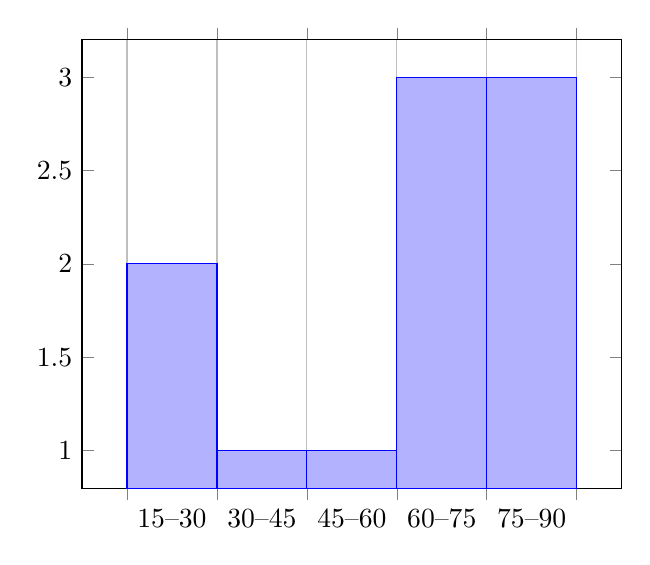
\begin{tikzpicture}
\begin{axis}[
            ybar interval,
            xticklabel=
\pgfmathprintnumber\tick--\pgfmathprintnumber\nexttick
        ]
\addplot+[hist={bins=5}]
            table[row sep=\\,y index=0] {
            data\\
            15\\ 72\\ 55\\ 29\\ 67\\ 89\\ 33\\ 65\\ 78\\ 90\\
            };
\end{axis}
\end{tikzpicture}
\end{figure}

\subsection{Steam and leaf plots}
% http://www.purplemath.com/modules/stemleaf.htm
% TODO describe how its useful to assist in visualizing the shape of a distribution
Steam and leaf plots (The left column of the stem and leaf plot represents the tens place; each number on the right side represents the ones place for the number of pairs of jeans at a department store.)
% TODO draw stem and leaf plot

Next, it must be determined what the stems will represent and what the leaves will represent. Typically, the leaf contains the last digit of the number and the stem contains all of the other digits. In the case of very large numbers, the data values may be rounded to a particular place value (such as the hundreds place) that will be used for the leaves. The remaining digits to the left of the rounded place value are used as the stem.

In this example, the leaf represents the ones place and the stem will represent the rest of the number (tens place and higher).

\section{Standard Data points}
When performing statistical analysis its often helpful to calculate a number of standard data points that helps uncover the nature of the data. Of these the mean, median and mode are all estimates of where the "middle" or "average" of the data is, once these values have been established we can take any observation and see how it relates to the average, for example if we have established that the everage grade is B then a student getting C is below average and a A student is above.

\begin{description}
\item [Mean] Is the sum of the observations divided by the number of observations e.g. the mean of $\{3, 3, 5, 9, 11\}$ is $(3 + 3 + 5 + 9 + 11)/5 = 6.2$. more formally suppose we have a data set containing the values $a_1,\ldots,a_n$, then the arithmetic mean $A$ is defined as
\begin{equation}
A = \frac{1}{n}\sum_{i=1}^{n} a_i
\end{equation}
\item [Median] The "middle" value of the numbers. To find the median arranging all the observations from lowest to highest and pick the middle one (e.g., the median of $\{3, 3, 5, 9, 11\}$ is $5$). If there is an even number of observations then the median is the mean of the two middle values (the median of $\{3, 5, 7, 9\}$ is $(5 + 7) / 2 = 6$).
\item [Mode] The "mode" is the value that occurs most often. If no number is repeated, then there is no mode. e.g. the mode of $\{3, 3, 5, 9, 11\}$ is $3$. In the data set:
$\{1, 1, 1, 2, 2, 2, 3\}$ we see that $1$ and $2$ both have the most occurrences, so they are both modes.
\end{description}

Two less frequently used values are the range and mid-range

\begin{description}
\item [Range] The "range" is the difference between the largest and smallest values. e.g. the range of $\{3, 3, 5, 9, 11\}$ is $11-3=8$.
\item [Mid-range] the mid-range is the arithmetic mean of the maximum and minimum values in a data set
\[
\textrm{MidRange} = \frac{min(x) + max(x)}{2}
\]
\end{description}

% TODO describe their usages
The standard deviation is the average distance between the actual data and the mean.

\subsection{Quartiles}
When using histograms for data analysis we may split the data into any number of groups we deem necessary. This arbitrary split can lead to results that are hard to compare as different researchers may group their data differently. Thus to compare data its useful to group data using a stansafized method, one such method is that of quartiles. With quartiles the data is split into four groups, known as a quartile. Each quartile contains $25\%$ of the total observations. Generally, the data is ordered from smallest to largest with those observations falling below $25\%$ of all the data analysed allocated within the $1st$ quartile, observations falling between $25.1\%$ and $50\%$ and allocated in the $2nd$ quartile, then the observations falling between $51\%$ and $75\%$ allocated in the $3rd$ quartile, and finally the remaining observations allocated in the $4th$ quartile.

When splitting data sets into their quartiles we do so by calculating the boundary values of each quartile known as $Q_1$, $Q_2$ and $Q_3$. Such that

% TODO check this is correct
\begin{itemize}
\item $1st$ quartile $v \in S \text{ where } v < Q_1$
\item $2nd$ quartile $v \in S \text{ where } v > Q_1 \text{ and } v < Q_2$
\item $3rd$ quartile $v \in S \text{ where } v > Q_2 \text{ and } v < Q_3$
\item $4th$ quartile $v \in S \text{ where } v > Q_3$
\end{itemize}

to calculate these we use the following method
\begin{enumerate}\label{stat:quartiles}
    \item Sort data values and find its median, This is $Q_1$.
    \item Divide the data set into two groups: a low group and a high group. When n is odd, the median should be placed in both groups.
    \item Find the median of the low group. This is $Q_1$.
    \item Find the median)of the high group. This is $Q_3$.
\end{enumerate}

Once the quartiles have been determined, its common to calculate the inter-quartile range (IQR)
\begin{equation}
IQR = Q_3 - Q_1
\end{equation}
% TODO why is this useful
A good summary of locations in the distribution is provided by the points that divide the data it into four equally-sized groups. This is the 5-point summary is made of:
\begin{enumerate}
    \item Quartile 0 the minimum
    \item Quartile 1 (bigger than 25\% of the data points)
    \item Quartile 2 (the median)
    \item Quartile 3 (bigger than 75\% of the data points)
    \item Quartile 4 (the maximum)
\end{enumerate}
The five-number summary gives information about the location (from the median), spread (from the quartiles) and range (from the sample minimum and maximum) of the observations
% TODO why is this useful

For example the data set $\{0, 1.5, 2.5, 3, 4, 4, 4, 7, 7.5\}$ has the median $4 = Q_2$. The data to the left of the median is $\{0, 1.5, 2.5, 3\}$ which has $2 = Q_1$ as its median. The data to the right is $\{4, 4, 7, 7.5\}$ which has $5.5 = Q_3$ as its median.

% TODO explain box plots

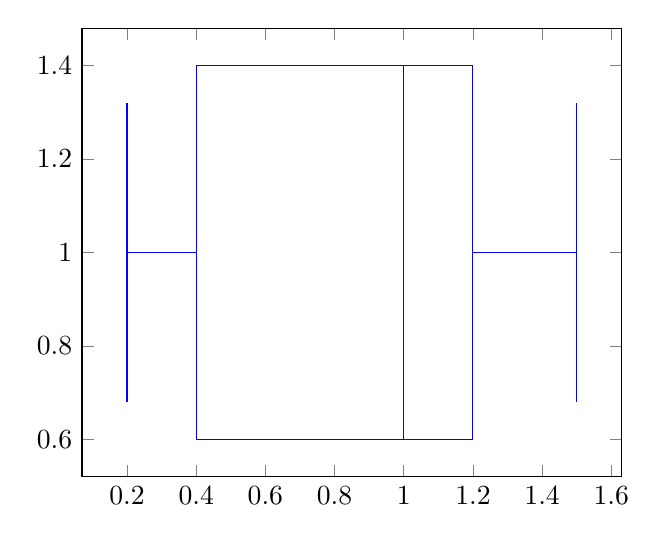
\begin{tikzpicture}
  \begin{axis}
    \addplot+[
    boxplot prepared={
      median=1,
      upper quartile=1.2,
      lower quartile=0.4,
      upper whisker=1.5,
      lower whisker=0.2
    },
    ] coordinates {};
  \end{axis}
\end{tikzpicture}

\subsection{Distributions}
% TODO http://en.wikipedia.org/wiki/Statistical_dispersion
% TODO draw examples of the different dsitributions
% TODO (symetrical/asymetrical)
% skewed (skewed to the right = right tailed, skewed to the left = left tailex )
% TODO http://stattrek.com/statistics/charts/data-patterns.aspx clusters, gaps, peeks, outliers
% - peek: value where most observations occur
% - gap: a range of values where no observations occur
% - cluster: a group of observatiins sepearetd from other observatiins by gaps
% - outlier: observations seperated by gaps from the main distribution

\subsection{Deviation and variance}
deviation is a measure of difference between the observed value of a variable and some other value, often that variable's mean

% TODO Average absolute deviation http://en.wikipedia.org/wiki/Absolute_deviation#Average_absolute_deviation_.28general_form.29
% TODO mean and median absolute diviation http://en.wikipedia.org/wiki/Median_absolute_deviation
% TODO (Why Square?) http://www.mathsisfun.com/data/standard-deviation.html#WhySquare
% TODO describe usage of and when to use
\begin{description}
    \item [Mean absolute deviation] The mean of the distances of each value from their mean.
\begin{enumerate}
    \item Find the mean of all values
    \item Find the distance of each value from that mean (subtract the mean from each value, ignore minus signs
    \item Then find the mean of those distances
\end{enumerate} For example the Mean Deviation of $3, 6, 6, 7, 8, 11, 15, 16$ is $3.75$ as the mean is $9$ and the distances from this are $6, 3, 3, 2, 1, 2, 6, 7$
\end{description}

The Variance is defined as:

The average of the squared differences from the Mean.

To calculate the variance follow these steps:

Work out the Mean (the simple average of the numbers)
Then for each number: subtract the Mean and square the result (the squared difference).
Then work out the average of those squared differences.

% TODO standard deviation

\section{Regression}
Regression is the main statistical technique used to quantify the relationship between two or more variables. A regression analysis would show a positive relationship between height and weight, for example. The measure of the accuracy of a regression is called R-squared. A perfect relationship, with no error, would have an R-squared of $1.00$ or $100$. Strong relationships, like height and weight, would have an R-squared of around $70$ percent. A meaningless relationship, like hair color and weight, would have an R-squared of zero.

\section{Random samples}
A random sample of $25\%$ of a schools pupules shoved that 16 pupiles had red hair. Based on the data, what is the most reasonable estimate of the total number of pupiles with red hair on the school?. $25\%$ is the same as $1/4$ of the pupiles at the school so the most resonable estimate is $4$ times the number from the sample $4 \cdot 16 = 62$

\section{Exercises}
\begin{ExerciseList}

% TODO MEAN, MEDIAN and MODE excercises

\Exercise Calculate the quartiles of the following data sets
\Question $\{0, 0, 1, 2, 2, 3, 3, 4\}$
\Question $\{3, 4, 4, 5, 5, 5, 6, 7\}$
\Question $\{7, 9, 9, 10, 10, 10, 11, 12, 12, 14\}$
\Question $\{0, 1, 1, 3, 3, 3, 4, 5, 7\}$
\Answer As described in \ref{stat:quartiles} we first calculate $Q_2$ and use its value to find $Q_1$ and $Q_3$
\begin{enumerate}
\item \myindent $Q_2 = 2, Q_1 = 1/2, Q_3 = 3$
\item \myindent $Q_2 = 5, Q_1 = 4, Q_3 = 5.5$
\item \myindent $Q_2 = 10, Q_1 = 9, Q_3 = 12$
\item \myindent $Q_2 = 3, Q_1 = 1, Q_3 = 4.5$
\end{enumerate}

\Exercise Use the normal distrubhtion to answer
\Question normally distributed random variable X has a mean of 20 and a standard deviation of 4. Determine the probability that a randomly selected x-value is between 15 and 22.
\Question The final exam scores in a statistics class were normally distributed with a mean of 58 and a standard deviation of 4. Find the probability that a randomly selected student scored more than 62 on the exam
\Answer TODO

\end{ExerciseList}


%\part{Advanced Mathematics}
%\chapter{Real analysis}
% TODO missing analysis terms
% - Fubini's theorem
The discovery of calculus by eighteenth century mathematicians, notably Newton
and Leibniz, was largely due to increased understanding of the behavior of real
functions. The birth of analysis is often traced to the early nineteenth century
work of Cauchy, who gave precise definitions of concepts such as continuity and
limits for real functions. Convergence problems while approximating real
functions by Fourier series gave rise to both the Riemann and Lebesgue
integrals. Cantor developed his set theory in an effort to answer uniqueness
questions about Fourier series

%\chapter{Abstract algebra}
% TODO missing abstract algebra
% - go through first math chapter of "Symbolic C++" (commutative group, distributive, ..)
% - explain why these defenitions are needed

\section{Groups}


\section{Rings and Fields}
A ring os a ordered triple $(R, +, \cdot)$ consisting of a set R with two
binary operations $+$ (addition) and $\cdot$ (multiplication), satiesfying the
folloiwn conditions

\begin{enumerate}
\item the pair $(R, +)$ is a commutative group
\item multiplication is associative
\item it admits an identity (or unit) element, denoted by $I$
\item multiplication is distributive on both sides over addition, i.e.
\[
x \cdot (y + z) = x \cdot y + x \cdot z
\textnormal{ and }
(x+y) \cdot z = x \cdot z + y \cdot z
\textnormal{ for all } x,y,z \in R
\]
\end{enumerate}

\noindent A subring of $R$ is a subset $S$ of $R$ satiesfying:
\begin{enumerate}
\item $S$ is a subgroup of the additive group $R$
\item $x \in $ and $y \in S$ together imply $x \cdot y \in S$
\item $I \in S$
\end{enumerate}
Thus a subring is a ring

If an element $a \in R$ posses an inverse element with respect to
multiplication, i.e. if there exists a (unique) $a^{-1} \in R$ such that
\[
a \cdot a^{-1} = a^{-1} \cdot a = I
\]
then we say that a is an \textit{invertible element} of R.

The set of invertible elements of a ring $R$ is denoted by $R^*$. If every
non-zero element of $R$ is invertible, rhen $R$ is sait to be a
\textit{division ring}. A commutative division ring is called a\textit{field}.
$S$ is a \textit{subfield} of $F$ is $S$ is a subring of $F$ and
$x \in S, x \neq 0$ together imply $x^-1 \in S$.

Examples of rings are $\mathbb{Z}, +, \cdot$ and $\mathbb{Q}, +, \cdot$. Where
$\mathbb{Z}$ is subring of $\mathbb{Q}$. The only invertible elements of
$\mathbb{Z}$ is $1$ and $-1$ whereas all non-zero elements of $\mathbb{Q}$ are
invertible.

\subsection{Polynomial ring}

%\chapter{Topology}
% TODO missing topology topics
% - Hausdorff space
% - Manifold
% - Furstenberg's proof of the infinitude of primes http://en.m.wikipedia.org/wiki/Furstenberg%27s_proof_of_the_infinitude_of_primes

A rubber band can be slipped off any place on a ball, a box, a bun,  or a blob without a hole, which makes them all essentially similar  or, in the language of topology, diffeomorphic to one another. This  means you can reshape any one of them into any other and then  back again.




%\chapter{Measure theory}
% TODO missing measure theory concepts
% - Lebesgue measure is the standard way of assigning a measure to subsets of n-dimensional Euclidean space. For n = 1, 2, or 3, it coincides with the standard measure of length, area, or volume
% http://terrytao.files.wordpress.com/2012/12/gsm-126-tao5-measure-book.pdf

One of the most fundamental concepts in Euclidean geometry is measuring 
geometric figures in one or more dimensions. In one, two, and three dimensions, 
we refer to their measure as the length, area, or volume of respectively.

With the advent of analytic geometry, however, Euclidean geometry became 
reinterpreted as the study of Cartesian products $\mathrm{R}^d$ of the real line 
$\mathrm{R}$. Using this analytic foundation rather than the classical geometrical 
one, it was no longer intuitively obvious how to define the measure $m(E)$ of a 
generall subset $E$ of $\mathrm{R}^d$;


%\chapter{Advanced statistics}
\section{Stochastic process}
% TODO http://planetmath.org/stochasticprocess

\subsection{Continuous-time Markov process}
%% Mathematica: http://reference.wolfram.com/language/ref/ContinuousMarkovProcess.html

\subsection{Discrete-time Markov process}
%% Mathematica: http://reference.wolfram.com/language/ref/DiscreteMarkovProcess.html

\subsection{Hidden Markov process}
%% Mathematica: http://reference.wolfram.com/language/ref/HiddenMarkovProcess.html

%\chapter{Non-Euclidean geometry}
% TODO missing non-euclidean geometry
% - History and motivation http://www-history.mcs.st-and.ac.uk/HistTopics/Non-Euclidean_geometry.html

\section{Projective geometry}

\section{Elliptic geometry}

\section{Hyperbolic geometry}

%\chapter{Differential geometry}

\section{Geodesics}

\section{Metric tensor}

\section{Riemann curvature}

%\include{subfiles/advanced/07_game_theory}

%\part{Mathematics in Finance}
%\chapter{Finance theory}
% TODO Missing finance concepts
%* simple imterest
% - present value under simple interst
% - interst paid at different time periods
%* compund interst
% - future value of compund intersts
% - calculation of the interst rate
% - present value under compund interst
%* interst rate
% - nominal and effective interst rate and converting between them
%* Annuities
% - future and present value
% - periodic payment and future value of annuity
% Bonds
% http://www.investopedia.com/exam-guide/cfa-level-1/

% stock option
The idea of a stock option is that you purchase an option to buy stock at an agreed price prior to some fixed later date. If the value of the stock rises above the agreed price before the option runs out, you buy the stock at the agreed (lower) price. If you want, you can sell the stock immediately and realize your profit. If the stock does not rise above the agreed price, you don’t have to buy it, but you lose the money you used to purchase the option. What makes stock options attractive is that the purchaser knows in advance what the maximum loss is: the cost of the option. The potential profit is theoretically limitless: The question is, What is a fair price to charge for an option on a particular stock?

Black-Scholes formula. (It was discovered by Scholes and Black and developed by Merton.) This formula tells investors what value to put on a financial derivative, such as a stock option. By turning what had previously been a guessing game into a mathematical science. the Black-Scholes formula does not eliminate uncertainty; it merely helps us to judge the risks.

The formula takes four input variables—duration of the option, prices, interest rates, and market volatility—and produces a price that should be charged for the option. 

% TODO add functions to Solvr

\section{The time value of money}
We all know that money deposited into a savings account will earn interest.
Because of this ability we prefer to receive money today rather than the same
amount in the future (since if we recived it today it could earn interest and therefor be worth more than the same amount recived in the future). This simple
fact about money is the corner stone of all mthemtical finance theory and is
known as the "time value of money". For example, assuming a $5\%$ interest rate,
$100$ invested today will be worth $105$ in one year ($100$ multiplied by $1.05$).
Conversely, $100$ received one year from now is only worth $95.24$ today ($100$
divided by $1.05$).

\subsection{Interests}
When money is lent, borrowed or invested interest ($I$) is paid. The interest
paid is determined by three factors

\begin{enumerate}
    \item Amount borrowed (known as the principle or capital ammont)
    \item Length of time for which money is borrowed
    \item The rate at which interest is charged
\end{enumerate}

Interest is calculated by dividing the total time into periods (days, weeks,
months, quarters, half- years, years etc). For each period the money earns
interest. At the end of these periods the money is worth the original (P)
amount plus interest (I). This new amount will be referred to as the Future
Value (FV). The number of periods will be referred to as (N).

Interest can be simple by letting the principal stay the same after each
interest peiod
\[
    SimpleInterest(P,j,t) = P*(1+j*t)
\]
or it can be compund by adding the accrued interest to the principal e.g.
\[
    CompundInterest(P,j,m,t) = P*(1 + j/m)^(t*m)
\]

The present value, is a future amount of money that has been discounted to
reflect its current value, as if it existed today.
\[
    PresentValue(S,j,m,t) = S/((1 + j/m)^(t*m))
\]

%\chapter{Actuarial mathematics}
Until the beginning of the 1980s, the concept of a pension was largely synonymous with the idea of a defined benefit (DB) plan; that is, the promise of a pension meant that upon retirement, an individual would receive a predetermined amount for the rest of his or her life.

Beginning in the 1980s, there was substantial growth in defined contribution (DC) plans. In these plans, the employer does not specify what benefits the retiree will receive. Instead, an investment account is opened for an employee, the employer and/or the employee make contributions to it, and upon retirement the individual can draw upon the money in the account.

Depending on how much is contributed and how well it is invested, the retiree could have more than enough for a comfortable retirement, or less than enough.

Assume you enter the labor force at the age of 35. Your job pays a fixed 50,000 per year for the next thirty years, after which you retire at age 65. This job provides no pension instead its your responsibility to ensure you save enough to maintain a dignified standard of living during your retirement. Finally also ignore taxes (both income tax and any possible deductions earned from participating in a pension plan) and we assume you die at age 95.

\section{Probability models of mortality}
As described above the  the key metric in a retirement scheme is how long people live, to ensure the pension plan is fully funded. If we are willing to stretch our idea of "experiment" the length of life may be considered a variable experiment result since people living under similar conditions will die at different unpredictable ages.

% notes
You probably see life insurance as a way to avoid having to worry about what will happen to your loved ones if you die. The insurance companies see it as a bet on how long you will live. As a business, they have to bet in such a way that their expectation is sufficiently positive for them to make an adequate profit.

Since the only framework available for discussing probabilities was games of chance, Christiaan Huygens conceived a life table as a lottery having 100 tickets of different values corresponding to the table’s entries. He then proceeded to calculate life expectancies using the rule for computing expectation that he had given in his earlier paper. For example, he stated that the number of chances that a person aged sixteen will die before age thirty-six equals 24, and that the number of chances that he will die after age thirty-six equals 16. Thus, in a fair game, you should bet 16 to 24, that is, 2 to 3, that the sixteen-year-old will die before age thirty-six.
.

%\part{Mathematics in Physics}
%\chapter{Classical mechanics}
% 1653 Pascal’s law of pressure.
% electromagnetism
% brownian motion
%\chapter{Relativity}

\section{Special relativity}
\subsection{Lorentz transformations}

\section{General relativity}


% appendices
\appendix
\chapter{Solutions to the exercises}
Each exercise is numbered in accordance with the chapter where it is to be found, thus exercise two in chapter one is referred to as $1.2$.
\shipoutAnswer

% index
\backmatter
\printindex

\end{document}

% Notes
% - remember orientation as english is read left (venstre) to right (Højre)
